% !TeX program = pdflatex
% !BIB program = bibtex
%%
%% Expert Systems with Applications — Manuscript (Double-Column, CAS)
%% Double-anonymized peer review: NO author names, affiliations, or acknowledgements in this file.
%%
\documentclass[a4paper,fleqn]{cas-dc}

% ESWA author-year citations use the abbreviated author list in running text
% (e.g., Ouyang et al., 2022), including the first occurrence.
\usepackage[authoryear]{natbib}

\usepackage{booktabs}      % professional tables
\usepackage{multirow}      % table row merging
\usepackage{array}         % flexible table column definitions
\usepackage{tabularx}      % auto-width table columns
\usepackage{hyperref}      % clickable references
\usepackage{microtype}     % better text justification
\usepackage{amsmath,amssymb} % math
\usepackage{graphicx}
\usepackage{capt-of}       % non-floating caption support for verification tables

% Keep the submission source engine-neutral. The manuscript is entirely in
% English, so loading CJK/fontspec support only changes the CAS font stack and
% can produce inconsistent metrics across online TeX installations.

% Some CAS installations leave \columnwidth at \textwidth after the title
% material. Restoring the dimensions explicitly prevents full-width paragraphs
% from being poured into the two-column output routine and overlapping.
\newcommand{\restorecasdoublecolumn}{%
  \normalfont
  \setlength{\columnsep}{18pt}% official cas-dc value
  \setlength{\columnwidth}{\dimexpr(\textwidth-\columnsep)/2\relax}%
  \setlength{\hsize}{\columnwidth}%
  \setlength{\linewidth}{\columnwidth}%
}

% ── Suppress author-info commands (double-blind) ──────────────────────────────
\begin{document}
\let\WriteBookmarks\relax
% cas-common prints an empty ORCID footnote even for this double-blind draft.
% Suppress the placeholder and its associated footnote rule.
\renewcommand{\printorcid}{}
\def\floatpagepagefraction{1}
\def\textpagefraction{.001}

% ── Relax float placement so figures stay near their call-site ────────────────

% Running header
\shorttitle{Multi-Agent Collaborative QA: A Survey}
\shortauthors{Anonymous}

% ── Title ─────────────────────────────────────────────────────────────────────
\title[mode=title]{%
  Multi-Agent Collaborative Question Answering Systems Based on Large Language
  Models: A Comprehensive Survey}

% ── Abstract ──────────────────────────────────────────────────────────────────
% Word limit: 250 words. NO references, NO abbreviations without definition.
\begin{abstract}
Large language models (LLMs) have enabled question answering (QA) systems to
use multiple interacting agents, but evidence about when collaboration is
useful remains fragmented. This paper presents a structured evidence-mapping
review of multi-agent collaborative QA using 78 cited sources from an
85-record bibliography pool, with 14 studies coded as core or boundary-case
evidence published through July 2026. We first
classify systems by the distribution of decision authority and control into
flat, hierarchical, and hybrid architectures. We then develop a qualitative,
two-phase architecture-selection approach that uses task complexity and
domain span, process standardisation and dynamism, cost and resource burden,
and risk tolerance and auditability as its criteria. A diagnostic comparison
with ten published systems shows that the approach makes design assumptions
explicit while also exposing cases in which competing requirements make a
single categorical assignment inadequate.

The review further examines five enabling dimensions---agent communication,
task decomposition and scheduling, knowledge management, memory management,
and reasoning mechanisms. It organizes development and evaluation resources
into foundation components, orchestration frameworks, application resources,
and benchmarks and evaluation tools. The survey distinguishes answer-level
performance from collaboration-process quality and identifies priorities for
architecture-aware selection, joint coordination, provenance-aware knowledge
and memory management, mechanism-level evaluation, human--agent collaboration,
and continual learning. The selection approach is therefore
presented as a transparent screening device, not as an externally validated
performance model or a universal recommendation for multi-agent QA.
\end{abstract}

% ── Highlights ────────────────────────────────────────────────────────────────
% 3-5 bullet points; each MUST be ≤ 85 characters including spaces.
% ── Keywords ──────────────────────────────────────────────────────────────────
% 1-7 keywords, separated by \sep
\begin{keywords}
  Multi-agent systems \sep
  Question answering \sep
  Large language models \sep
  LLM agents \sep
  Retrieval-augmented generation \sep
  Survey
\end{keywords}

\maketitle

% Defensive reset for consistent cas-dc output on TeXPage and local systems.
\restorecasdoublecolumn
\setlength{\emergencystretch}{1em}

% Keep wide figures and tables near their discussion without creating a float
% backlog or large vertical gaps.
\renewcommand{\topfraction}{0.95}
\renewcommand{\bottomfraction}{0.90}
\renewcommand{\textfraction}{0.07}
\renewcommand{\floatpagefraction}{0.80}
\renewcommand{\dbltopfraction}{0.95}
\renewcommand{\dblfloatpagefraction}{0.80}
\setlength{\textfloatsep}{14pt plus 3pt minus 3pt}
\setlength{\floatsep}{12pt plus 3pt minus 2pt}
\setlength{\dbltextfloatsep}{14pt plus 3pt minus 3pt}
\setlength{\dblfloatsep}{12pt plus 3pt minus 2pt}

% ==============================================================================
% 1.  INTRODUCTION
% ==============================================================================
\section{Introduction}
\label{sec:intro}

Automatic question answering (QA) systems aim to enable users to pose
natural-language questions and receive accurate, concise answers
from a computer system.
From early rule-based expert systems to modern deep-learning architectures
grounded in information retrieval and machine reading comprehension, QA
has undergone a remarkable transformation.
In recent years, large language models (LLMs) such as GPT series
\citep{brown2020gpt3} \citep{openai2023gpt4} have demonstrated
strong natural-language understanding and generation capabilities relevant
to QA.
Nevertheless, QA systems built on a single LLM agent continue to face
fundamental limitations.
\emph{First}, single agents are prone to hallucination, producing factually
incorrect outputs with high confidence.
\emph{Second}, finite context windows impede reliable reasoning over long
documents or multi-hop inference chains.
\emph{Third}, a monolithic model cannot simultaneously possess expert-level
knowledge across all domains, often failing on queries that require
cross-disciplinary collaboration.

At the same time, multi-agent collaborative paradigms have
emerged, drawing theoretical inspiration from Minsky's ``Society of
Mind'' \citep{minsky1988society} and the formal foundations of multi-agent
systems \citep{wooldridge1995intelligent}.
Between 2023 and 2026 this field has witnessed explosive growth. For example,
influential frameworks such as AutoGen \citep{wu2024autogen} and MetaGPT
\citep{hong2024metagpt} illustrate the emergence of explicit multi-agent
coordination.
Through role specialization, mutual debate \citep{du2024multiagent_debate},
and structured task decomposition, multi-agent systems can improve answer
verification and task performance.

Existing surveys cover general LLM-agent construction, communication,
and orchestration
\citep{guo2024llm_multiagent_survey,tran2025multiagent_survey,wang2024survey_autonomous_agents}.
This survey builds on that coverage by connecting collaboration topologies and enabling mechanisms
to QA-specific task and governance requirements and architecture-selection
trade-offs through five related contributions:

\begin{enumerate}
  \item We construct a structured evidence map of multi-agent collaborative
        QA, based on a source-checked corpus with explicit roles for core empirical
        studies, supporting research, background literature, and technical
        documentation. The review distinguishes direct QA evidence from
        adjacent agent applications.
  \item We develop an operational architecture account that classifies
        systems by decision authority and control into \textbf{flat},
        \textbf{hierarchical}, and \textbf{hybrid} patterns, and combines the
        taxonomy with a qualitative, two-phase selection approach. The approach
        uses a single-agent baseline, explicit decision criteria, and a
        diagnostic comparison with ten published systems to identify its
        boundary conditions.
  \item We synthesize five technical dimensions that support collaborative QA:
        agent communication, task decomposition and scheduling, knowledge
        management, memory management, and reasoning mechanisms. The discussion
        distinguishes the functions and trade-offs of these mechanisms rather
        than treating them as interchangeable capabilities.
  \item We organize development and evaluation resources into four layers:
        foundation components, orchestration frameworks, application
        resources, and benchmarks and evaluation tools. This map clarifies the
        distinction between implementation support, application configuration,
        and evidence for answer-level or collaboration-process performance.
  \item We synthesize open challenges and future research directions around
        architecture adaptation, communication and task coordination, knowledge
        and memory lifecycle, reasoning-process evaluation, human--agent
        collaboration, and continual learning.
\end{enumerate}

The remainder of the paper follows this logic. Section~3 presents the
architecture taxonomy and selection approach; Section~4 reviews the enabling
technologies; Section~5 organizes development and evaluation resources; and
Section~6 discusses open challenges and future directions.

% ── 1.1  Literature identification and evidence roles ─────────────────────────
\subsection{Literature search and evidence-mapping protocol}
\label{sec:slr}

\subsubsection{Corpus construction and verification}
\label{sec:search}

This survey uses a \emph{structured evidence-mapping review}. It does not seek to conduct an exhaustive PRISMA-style systematic review, as its objective is to synthesize multiple types of sources—empirical multi-agent QA studies, related agent research, foundational literature, and evolving technical documentation—with explicitly defined roles for each category of evidence.

The historical audit log records an initial candidate set of 108 unique
entries from the authors' working bibliography and checks dated 2 August
2026 using Crossref, OpenAlex, arXiv, and official sources. It records four
corrupted or mismatched records for which an authoritative source was not
confirmed, together with duplicate, uncited, and out-of-scope records. These
historical records are retained in the audit trail; the log alone is not
independent evidence that every publication field was verified.

The historical targeted update used combinations of \textit{multi-agent},
\textit{LLM}, \textit{question answering}, \textit{reasoning},
\textit{long-context}, and \textit{retrieval-augmented generation} across the ACL
Anthology, OpenReview, arXiv, and publisher proceedings. It added ReConcile
\citep{chen2024reconcile}, Chain-of-Agents \citep{zhang2024chain_agents}, and
CoCoA \citep{jiang2026cocoa}.

A source-level recheck on 8 October 2026 compared the 84-record bibliography
pool with publisher records, official proceedings, versioned arXiv papers,
and project documentation. The accompanying audit separates source existence,
field accuracy, version conflicts, and claim support. Confirmed corrections
were applied, while inaccessible fields and unresolved conflicts remain
explicitly marked. One official LangGraph article was added to support the
specific interrupt and checkpoint mechanisms discussed below.

% Ensure that the monospace file-name style above cannot leak into subsequent
% headings or body text on TeX installations with older CAS dependencies.
\par\normalfont\normalsize
\subsubsection{Eligibility criteria and evidence classification}
\label{sec:screening}

The core eligibility screen (role \textbf{I}) used five criteria:
(1) publication from January 2019 through July 2026;
(2) an LLM serving as the primary agent backbone;
(3) at least two agents equipped with an explicit collaboration mechanism;
(4) QA, retrieval-augmented answering, conversational QA, or question-driven domain decision support as the primary evaluated task; and
(5) a described method or system accompanied by empirical evaluation. When both a preprint and a peer-reviewed version of a work existed, the peer-reviewed final publication was preferred.

Sources that informed collaboration mechanisms or applications but did not meet every core criterion were coded as supporting studies (role \textbf{S}).
Foundational models, datasets, single-agent methods, and review articles were coded as background (role \textbf{B}); official protocols and software documentation were coded as technical sources (role \textbf{T}).
Historically excluded sources remain coded as \textbf{X} in the audit file.
The current bibliography pool contains 85 records: 14~I, 16~S, 46~B, and
9~T. The effective manuscript cites 78 of these records: 14~I, 14~S, 42~B,
and 8~T; seven uncited records remain in the pool. The 14 role-I labels are
inherited author coding. Triad uses one LLM in three roles and is retained as
a boundary case pending an eligibility decision, rather than treated as
unambiguous evidence of multiple independent agents. Table~\ref{tab:validation}
identifies that boundary in the diagnostic comparison. Other claims use
sources appropriate to their scope. Fig.~\ref{fig:reference_corpus} retains
the earlier corpus snapshot; its counts require synchronization with this
corrected text.

\begin{figure*}[pos=t]
  \centering
  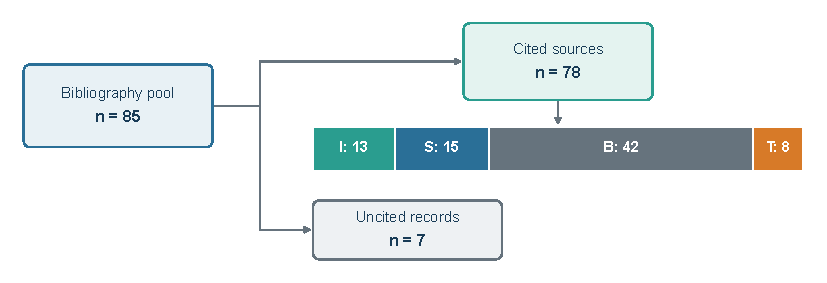
\includegraphics[width=0.80\linewidth]{fig_reference_corpus.pdf}
  \caption{Historical reference-corpus verification and evidence-role allocation. The figure retains the earlier 84-record snapshot; current pool and citation counts are given in the text. This is not an exhaustive PRISMA screening flow.}
  \label{fig:reference_corpus}
\end{figure*}

\section{Background: automatic QA and LLM-based agents}
\label{sec:background}

\subsection{Overview of automatic QA systems}
\label{sec:qa_overview}

Automatic question answering is a core branch of natural language processing (NLP) that interprets a user’s information need and generates an answer. Its major paradigms, including rule-based and knowledge-base QA, information-retrieval (IR) QA, machine reading comprehension (MRC), retrieval-augmented generation (RAG), and LLM-based agentic QA, have accumulated rather than supplanted one another. They differ in their primary evidence sources, reasoning interfaces, and operational assumptions.
For example, dense retrieval enables open-domain evidence access
\citep{karpukhin2020dpr}, whereas RAG combines retrieved evidence with generative answering \citep{lewis2020rag}. Multi-agent systems introduce an explicit coordination layer when a task demands distributed retrieval, reasoning, verification, or tool use.
Accordingly, the historical overview in this section should be regarded as a collection of representative milestones, rather than a single linear sequence of superseded paradigms. QA has also expanded from single-turn, closed-domain scenarios to multi-turn and open-domain settings.
Benchmark datasets have been instrumental in driving research progress.
Representative examples include HotpotQA \citep{yang2018hotpotqa} for
multi-hop reasoning, Natural Questions \citep{kwiatkowski2019natural_questions}
derived from real search queries, and CoQA \citep{reddy2019coqa} and QuAC
\citep{choi2018quac} for conversational QA.
These resources have facilitated advances in retrieval, generation, and complex reasoning. The representative milestones are illustrated in
Fig.~\ref{fig:qa_timeline}.

\begin{figure*}[pos=t]
  \centering
  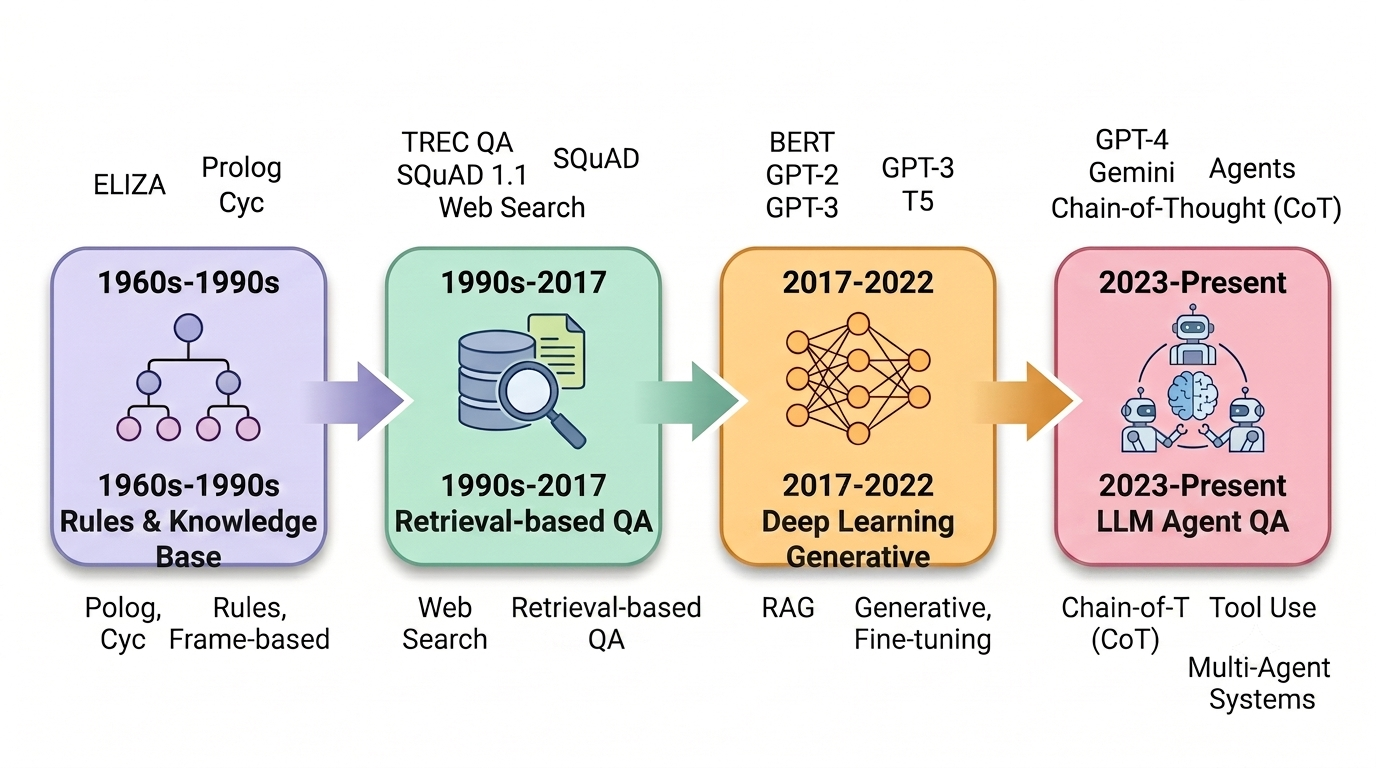
\includegraphics[width=0.82\textwidth]{change_timeline.jpg}
  \caption{Evolution timeline of automatic QA systems.}
  \label{fig:qa_timeline}
\end{figure*}

\subsection{LLM-based agents}
\label{sec:llm_agents}

\subsubsection{Core architecture of LLM-based agents}
\label{sec:agent_arch}

An LLM-based agent takes a large language model as its cognitive core and may be equipped with perception and action capabilities. For the analytical purposes of this review, we characterize agent functionality via four capabilities: \emph{Perception} (receiving environmental input), \emph{Planning} (task decomposition and goal setting), \emph{Action} (tool invocation and external interaction), and \emph{Memory} (short-term context management and long-term knowledge retrieval). This constitutes an analytical framework, rather than implying that every agent system implements these four identical components. For instance, ReAct specifically interleaves reasoning and action \citep{yao2023react}.
Formally, a multi-agent collaborative QA system can be defined as:
\begin{equation}
  \mathcal{S} = \langle \mathcal{A},\; \mathcal{C},\; \mathcal{T},\;
                \mathcal{E} \rangle
  \label{eq:mas_def}
\end{equation}
\noindent where $\mathcal{A} = \{a_1, a_2, \ldots, a_N\}$ is the set of
agents with each $a_i = \langle \pi_i, \mathcal{M}_i, \mathcal{K}_i
\rangle$ denoting its planning policy, memory state, and knowledge base;
$\mathcal{C}$ is the communication protocol; $\mathcal{T}$ is the task
space; and $\mathcal{E}$ is the shared execution environment.

The trajectory of LLM development has been decisive in enabling this architecture.
Representative milestones include the Transformer \citep{vaswani2017attention},
which introduced an attention-only sequence-transduction architecture; BERT
\citep{devlin2019bert}, which advanced bidirectional pretraining and
task-specific fine-tuning; and GPT-3 \citep{brown2020gpt3} and GPT-4
\citep{openai2023gpt4}, which demonstrated powerful few-shot and zero-shot
capabilities. Open-weight releases such as LLaMA \citep{touvron2023llama} and
ChatGLM \citep{glm2024chatglm} provide additional options for local
experimentation, while
InstructGPT \citep{ouyang2022instructgpt} exemplifies the use of Reinforcement
Learning from Human Feedback (RLHF) to improve instruction following.
Table~\ref{tab:llm_evolution} summarizes representative model capabilities relevant to agentic QA; this table serves as an illustrative overview rather than an exhaustive chronological record.


\clearpage
\onecolumn

\begin{table*}[pos=t]
  \centering
  \caption{Representative LLM capabilities relevant to agentic QA. Models
           were selected to illustrate capabilities used by agent systems,
           rather than to provide an exhaustive model history.}
  \label{tab:llm_evolution}
  \begin{tabular}{l c l p{7cm}}
    \toprule
    \textbf{Model} & \textbf{Year} & \textbf{Organisation} &
    \textbf{Capability relevant to agentic QA} \\
    \midrule
    BERT        & 2018  & Google  &
      Contextual language representations supporting language understanding \\
    GPT-3       & 2020  & OpenAI  &
      In-context learning for flexible task specification \\
    InstructGPT & 2022  & OpenAI  &
      Instruction following through RLHF-based alignment \\
    LLaMA series & 2023+ & Meta   &
      Open-weight model family supporting reproducible agent experimentation \\
    GPT-4       & 2023  & OpenAI  &
      Strong general reasoning and multimodal interaction capabilities \\
    ChatGLM series & 2023+ & THU/Zhipu &
      Bilingual and long-context capabilities for multilingual or document QA \\
    \bottomrule
  \end{tabular}
\end{table*}

\subsubsection{Rationale for the transition from single-agent to multi-agent systems}
\label{sec:motivation}

Single-agent architectures remain a strong baseline for tasks that can be
handled by one workflow, but their limitations become apparent when a problem
requires cross-domain knowledge, long-horizon reasoning, extensive evidence,
or high reliability. A single model must understand the query, retrieve and
assess evidence, generate an answer, and possibly verify its own output. This
concentration of functions creates three related risks: incomplete knowledge
and hallucination in unfamiliar domains, dilution of relevant evidence in long
contexts, and the absence of an independent perspective in a one-pass answer.
Self-refinement and tool use can mitigate these risks, but they do not remove
the underlying dependence on one model and one reasoning trajectory.

The motivation for multi-agent systems is therefore capability extension
rather than simple replacement. Inspired by Minsky's Society of Mind
\citep{minsky1988society}, multi-agent architectures can combine agents with
individual memory, reflection, and planning, as illustrated in social
simulations \citep{park2023generative_agents}. A single ``generalist'' workflow may combine
query understanding, retrieval, generation, and refinement, whereas a
multi-agent workflow can separate these functions into, for example, Planner,
Retriever, Generator, and Critic roles. MetaGPT demonstrates role allocation
among product managers, architects, and engineers in software development
\citep{hong2024metagpt}, while CAMEL studies sustained interaction between
user and assistant roles \citep{li2023camel}. These examples show how role
conditioning can structure collaboration, but they do not establish a
universal advantage: specialization is useful only when roles have genuinely
different information, tools, or verification responsibilities.

This division of labour can extend both knowledge coverage and effective
context capacity. Different agents may use complementary prompts, tools, or
evidence sources, so diversity is beneficial when it contributes independent
evidence rather than duplicated model calls. Likewise, segmenting a large
document across agents can support broader coverage than a single context,
as explored by LongAgent and Chain-of-Agents
\citep{zhao2024longagent,zhang2024chain_agents}. These gains are conditional:
intermediate results must still be communicated and synthesized, and
aggregation loss, communication cost, and the final synthesis context can
become new bottlenecks.

Multi-agent collaboration can also improve reasoning reliability by creating
separate candidate, review, and verification paths. Debate, cross-checking,
and reconciliation may expose errors that self-refinement within one workflow
overlooks \citep{du2024multiagent_debate,chen2024reconcile,
xiong2023inter_consistency}. However, additional agents do not guarantee
correctness: weak aggregation, poor interaction design, or correlated errors
can preserve or amplify an incorrect answer. Coordination quality is thus a
central design variable, not an incidental implementation detail.



% ==============================================================================
% SECTION 3: ARCHITECTURES OF MULTI-AGENT COLLABORATIVE QA SYSTEMS
% ==============================================================================
\section{Architectures of multi-agent collaborative QA systems}
\label{sec:architectures}

\subsection{Taxonomy of multi-agent collaborative QA architectures}
\label{sec:taxonomy}

This review classifies a collaborative QA system primarily by the distribution
of \emph{decision authority and control}. The classification  is based on the
workflow that routes subtasks, determines when an answer is accepted, and
controls final synthesis. A \textbf{flat} architecture has no persistent agent with top-down
authority over the other participants. A \textbf{hierarchical} architecture
assigns planning, routing, approval, or synthesis authority to one or more
managers, or imposes an ordered, asymmetric control flow across stages. A
\textbf{hybrid} architecture changes this authority structure across task
stages or decision states.  Other design considerations such as communication topology (for example, broadcast, peer exchange, or a graph),
role specialization, human-in-the-loop (HITL) checkpoints, and runtime routing are orthogonal attributes. For example, a group-chat framework is
not automatically flat, and a system with specialized roles is not automatically
hierarchical. The three classes are alternative control patterns rather than
stages of a historical progression. 
Figure~\ref{fig:topology}
provides an illustrative schematic.

\begin{figure*}[pos=t]
	\centering
	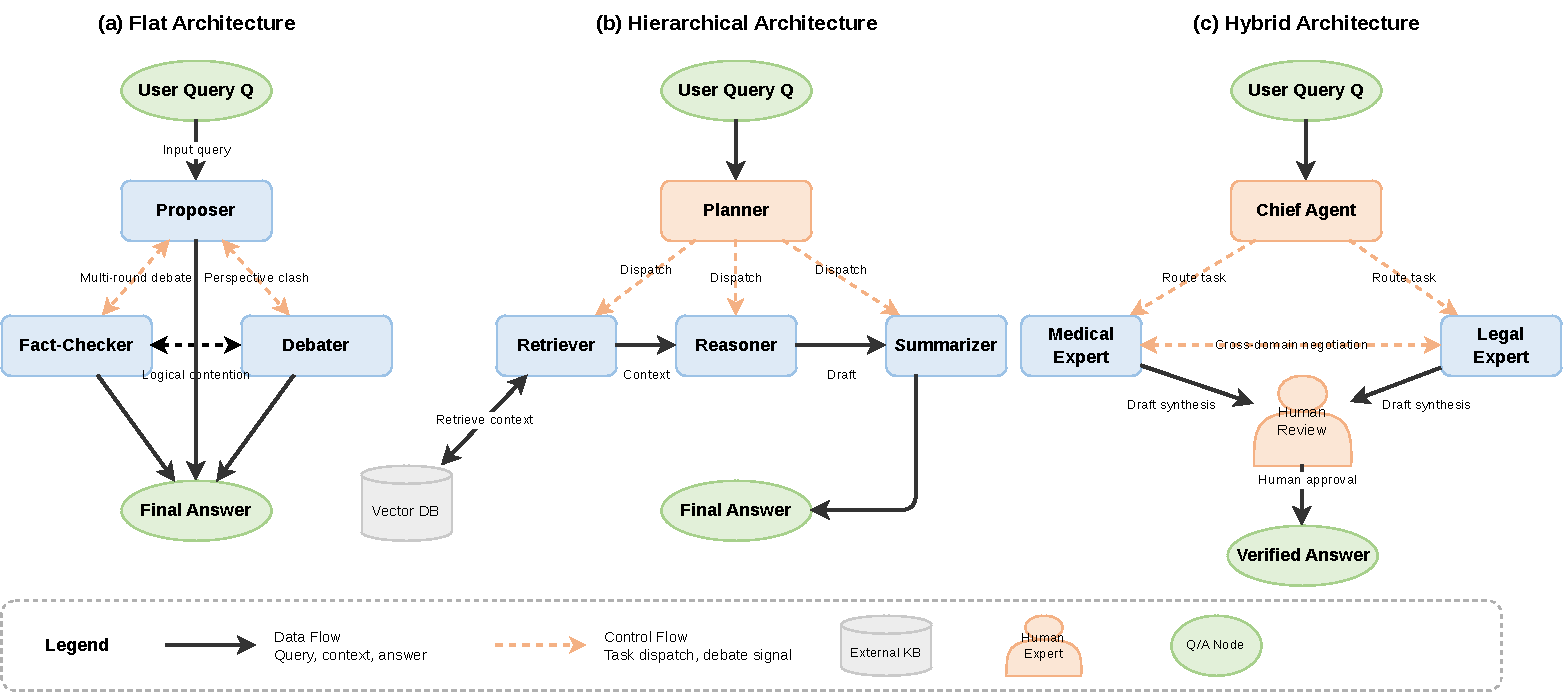
\includegraphics[width=\textwidth]{fig3_topology.pdf}
	\caption{Illustrative network topologies for multi-agent collaborative QA.
		The operational taxonomy is defined by decision authority and
		control, as specified in the text and Table~\ref{tab:9categories}.}
	\label{fig:topology}
\end{figure*}




\subsubsection{Flat architectures}
\label{sec:flat}

In a flat collaborative architecture, participating agents exchange information, critique candidate solutions, or engage in negotiations without a persistent top-down controller. The relevant characteristic lies in distributed decision-making authority, rather than unrestricted dialogue. A flat workflow may still enforce turn limits, adopt voting rules, or include a designated final aggregation step.

\paragraph{Multi-agent debate.}
\label{sec:debate}

In the multi-agent debate paradigm, several LLM agents generate candidate answers and critique one another across one or more rounds. Representative studies illustrate both the potential and the limits of this design. For example, \citet{du2024multiagent_debate} report improved factuality and reasoning performance on the tasks they evaluate, whereas divergent prompting can mitigate convergence toward similar reasoning paths \citep{liang2024divergent_debate}. ReConcile provides another example by integrating heterogeneous models with confidence-weighted consensus \citep{chen2024reconcile}; inter-model inconsistency and capability imbalance nevertheless remain important considerations \citep{xiong2023inter_consistency}. Accordingly, adding more agents or debate rounds does not reliably boost QA performance; instead, the interaction rules, diversity of evidence, and aggregation procedure determine whether disagreement yields correction, inconsistency, or unnecessary computational cost.

\paragraph{Role-conditioned collaboration.}
\label{sec:roleplay}

Role-conditioned collaboration assigns different prompts or task views to participating agents. For example, CAMEL \citep{li2023camel} employs an "AI User" and an "AI Assistant" paired with inception prompting to maintain role-conditioned interaction. This constitutes an adjacent multi-agent framework and does not serve as direct evidence that role playing improves QA accuracy. 

\paragraph{Group-chat collaboration.}
\label{sec:groupchat}

Group-chat collaboration adopts multi-participant conversations as its interaction interface. For example, AutoGen \citep{wu2024autogen} supports developer-defined speaker selection rules and conversation patterns instead of enforcing a fully flat, free-form group chat paradigm. Accordingly, its resulting topology is determined by application configurations. 

Flat architectures can be useful when independent viewpoints, mutual critique, or open-ended exploration are required. Their distributed structure can reduce reliance on a single reasoning path, yet it also incurs coordination costs.
In fully connected settings, the number of potential communication links grows quadratically with the number of agents. Additional rounds may introduce redundant context, delayed convergence, correlated errors, or pseudo-consensus.
By contrast, when tasks demand stable dependencies, predictable execution, or stringent cost control, explicit authority and routing mechanisms may be more appropriate.

\subsubsection{Hierarchical architectures}
\label{sec:hierarchical}

Hierarchical architectures delegate the authority for planning, routing, approval, or synthesis to one or more agents. Lower-level agents execute bounded subtasks or provide evidence to a manager. The workflow may take the form of a tree, a pipeline, or a controller–worker loop; its defining characteristic is asymmetric decision-making authority.

\paragraph{Manager--executor pattern.}
\label{sec:manager_executor}

The manager–executor pattern separates global planning from local execution.
For example, MetaGPT \citep{hong2024metagpt} adopts standard operating procedures and defines roles
including product manager, architect, and engineer. ChatDev \citep{qian2023chatdev}
provides another example by simulating a software development organisation via ChatChain. Both fall under related software engineering systems; they demonstrate structured delegation
yet do not provide direct evidence regarding QA performance. 

\paragraph{Plan--retrieve--generate pipeline.}
\label{sec:pipeline}

Knowledge-intensive QA can assign planning, retrieval, generation, and
verification to a staged workflow. Representative implementations include
LONGAGENT \citep{zhao2024longagent}, which coordinates a leader with
document-reading members; Chain-of-Agents \citep{zhang2024chain_agents},
which propagates information across context segments before synthesis; and
CoCoA-zero \citep{jiang2026cocoa}, which coordinates parametric and retrieved
knowledge using three agents at inference time. CoCoA subsequently distils
that collaboration into a single model. These role-I systems differ in their communication
and aggregation mechanisms, but each places subtask sequencing or synthesis
under explicit control. By contrast, HuggingGPT \citep{shen2024hugginggpt}
uses a controller to invoke specialised models and tools.




Hierarchical architectures can improve controllability by separating global planning from local execution. They are suitable for QA workflows with stable procedures, explicit dependencies, or quality-control checkpoints. However, this centralisation may introduce a planner bottleneck: an erroneous high-level plan can propagate errors, and rigid pipelines may fail to handle unexpected evidence or conflicting expert opinions. Therefore, the associated benefits depend on the quality of the controller and the availability of corrective pathways.

\subsubsection{Hybrid architectures}
\label{sec:hybrid}

Hybrid architectures alter the control configuration across task stages or decision states. A system may adopt peer deliberation to explore candidate solutions, hierarchical delegation to execute a selected plan, and conditional human oversight in scenarios where uncertainty or risk exceeds a predefined threshold. Simply combining individual components is insufficient; the coordination paradigm itself must be adaptive.

\paragraph{Graph-structured agent networks.}
\label{sec:graph}

Graph-structured networks represent agents and transitions as an executable graph. For example, LangGraph \citep{langgraph2024} serves as an official technical framework for defining state transitions, loops, and conditional branches; it provides technical evidence (role T), rather than constituting a QA evaluation. GPTSwarm \citep{zhuge2024gptswarm} provides another example through an empirical study of agent methodologies that optimises prompts and inter-agent graph connections. 

\paragraph{Adaptive collaboration-mode switching.}
\label{sec:adaptive}

Adaptive systems adjust team composition or control patterns as tasks evolve.
For example, AgentVerse \citep{chen2024agentverse} describes an iterative pipeline consisting of
expert recruitment, collaborative decision-making, action execution, and
result evaluation. This mechanism cannot be simplified to a "simple-flat/complex-
hierarchical" rule. MDAgents \citep{kim2024mdagents} provides direct
in-case evidence for adaptive medical collaboration. Such adaptive mechanisms
enhance routing flexibility, yet introduce extra requirements for state management
and performance evaluation.

\paragraph{Human-in-the-loop design pattern.}
\label{sec:hitl}

For example, LangGraph supports checkpointed state and pausing a workflow
with an interrupt for human review \citep{langgraph2024interrupt}, which may
be useful for high-risk decisions.

In a collaborative QA workflow, human participation can be placed at several
points: before task decomposition, after retrieval, when agents disagree, or
before an answer is released or an external action is executed. These points
serve different purposes. Early review can correct the interpretation of the
question and restrict the permitted tools; intermediate review can assess the
quality and provenance of retrieved evidence; and final review can provide an
approval boundary for consequential recommendations. The appropriate point is
therefore determined by the potential impact of an error and by the extent to
which the relevant state remains understandable and editable.

The reviewer should also have an explicitly defined level of authority. A
human may merely approve a proposed answer, select among agent outputs, edit
evidence or intermediate conclusions, or redirect the workflow by requesting
another retrieval or specialist analysis. These forms of participation are
not equivalent: approval without access to the supporting evidence provides
limited control, whereas unrestricted editing can make the origin of the
final answer difficult to reconstruct. A useful HITL design should preserve
the question, retrieved sources, agent contributions, reviewer intervention,
and resulting state transition in an auditable record.

HITL checkpoints can improve accountability and provide a recovery path when
agents encounter uncertainty, conflicting evidence, or unsafe requests. They
also introduce review latency, operator workload, and the possibility of
inconsistent decisions across reviewers. For this reason, a fixed human
breakpoint is not automatically preferable to automated execution. Risk-
adaptive policies that trigger review using uncertainty, disagreement,
evidence quality, or action impact are a plausible design, but their effects
on error interception, workload, and answer quality require empirical
evaluation. The current literature therefore supports HITL as a control
pattern and design objective, rather than as established evidence of safer QA
performance.



Hybrid architectures are useful when task requirements are heterogeneous or when the workflow must combine deliberation, controlled execution, and conditional review. Their trade-off lies in engineering complexity: dynamic routing, state transitions, and cross-mode information transfer are more difficult to configure, debug, evaluate, and reproduce. A hybrid design is justified when this additional adaptability addresses documented uncertainty or risk, rather than serving as a default replacement for fixed control patterns.

\subsubsection{Comparative discussion of architecture types}
\label{sec:arch_comparison}

Table~\ref{tab:9categories} compares the three architecture classes and their
sub-paradigms in terms of control, task suitability, and limitations.
Architecture labels, suitable contexts, and limitations are the authors'
synthesis of the cited mechanisms.

\begin{table*}[pos=t]
  \centering
  \caption{Comparison of multi-agent collaborative QA architecture classes.}
  \label{tab:9categories}
  \scriptsize
  \begin{tabular}{p{1.4cm} p{2.0cm} p{2.4cm}  p{3.2cm} p{2.3cm} p{2.2cm}}
    \toprule
    \textbf{Architecture} & \textbf{Sub-paradigm} &
    \textbf{Representative systems} &
    \textbf{Coordination and control} &
    \textbf{Suitable contexts} & \textbf{Limitations} \\
    \midrule
    \multirow{3}{*}{\textbf{Flat}} &
    Multi-agent debate & \citet{du2024multiagent_debate} & 
    Peer critique and aggregation can add independent answer paths &
    Tasks needing competing factual or reasoning views &
    Coordination cost and aggregation sensitivity \\
    & Role-conditioned collaboration & CAMEL \citep{li2023camel} & 
    Personas structure interaction but do not by themselves establish QA gains &
    Exploratory collaboration and prompt-role studies &
    Fixed roles or correlated perspectives \\
    & Group-chat collaboration & AutoGen \citep{wu2024autogen}  &
    Developer-defined speaker selection and dialogue patterns &
    Applications requiring configurable conversations &
    Topology and QA performance depend on configuration \\
    \midrule
    \multirow{3}{*}{\textbf{Hierarchical}} &
    Manager--executor pattern & MetaGPT \citep{hong2024metagpt}  &
    Manager assigns staged work to specialised executors &
    Structured engineering workflows &
    Planner bottleneck and error propagation \\
    & Staged evidence-processing pipeline & LONGAGENT; Chain-of-Agents; CoCoA-zero
    \citep{zhao2024longagent,zhang2024chain_agents,jiang2026cocoa}  &
    Explicit sequencing and final synthesis over distributed evidence &
    Long-document or knowledge-intensive QA &
    Information loss and coordination cost at synthesis \\
   
    \midrule
    \multirow{3}{*}{\textbf{Hybrid}} &
    Graph-structured agent networks & GPTSwarm; LangGraph
    \citep{zhuge2024gptswarm,langgraph2024}  &
    DAG connection optimization in GPTSwarm; loops and conditional routing in LangGraph &
    Workflows with conditional state transitions &
    Different evidence roles; difficult debugging and tracing \\
    & Adaptive collaboration-mode switching & MDAgents \citep{kim2024mdagents}  &
    Changes collaboration in response to case characteristics &
    Tasks with heterogeneous requirements &
    Routing policy must be evaluated, not assumed beneficial \\
    & Human-in-the-loop design pattern & LangGraph interrupts \citep{langgraph2024interrupt} &
    Human review at explicitly defined decision points &
    High-risk workflows requiring accountability &
    Direct comparative QA evidence remains limited \\
    \bottomrule
  \end{tabular}
\end{table*}

These architecture types differ in where decision authority is placed and when it
changes. Communication topology remains a useful secondary descriptor, but it
does not supersede the operational rules above. 
% ── 3.2  Architecture Selection Approach ────────────────────────────────────
\subsection{Architecture selection approach}
\label{sec:guideline}

The taxonomy describes alternative control patterns; it does not imply that
multi-agent collaboration is preferable for every QA task. Architecture
selection must also account for the task, process, resource, and governance
conditions under which collaboration is justified. The approach below treats a
single-agent workflow as a valid baseline and produces a reasoned shortlist of
candidate architectures rather than a universal assignment.

\subsubsection{Scope and selection criteria}
\label{sec:framework_scope}

Four criteria connect task requirements to the control patterns in the
taxonomy. They support transparent comparison across studies, but do not
define universal numerical thresholds or claim that one architecture
dominates the others.

\textbf{1. Task complexity and domain span.} The analysis starts from the
reasoning structure, evidence requirements, output criteria, and domain span.
The criterion captures the number and interdependence of reasoning steps, the
breadth of required expertise, and the need for independent evidence sources.
Single-agent execution is often adequate for short, low-uncertainty queries;
decomposition and role specialization become more plausible when a task
combines separable subtasks or domains. Complexity alone, however, does not
establish that additional agents will improve the answer: each role must
contribute distinct information or checks.

\textbf{2. Process standardization and dynamism.} Stable stages and explicit
dependencies favor hierarchical or pipeline control, whereas open-ended tasks
may benefit from peer generation and critique. When the appropriate mode
changes across queries or stages, hybrid routing is a candidate design. These
are tendencies rather than deterministic mappings: hierarchical workflows can
contain local debate, and flat workflows can enforce turn limits and
aggregation rules.

\textbf{3. Cost and resource burden.} Multi-agent execution adds
communication, aggregation, state-management, and inference costs. Reported
multi-agent failure modes \citep{han2024mast} motivate checking whether
additional coordination provides useful benefits. As a design criterion,
this review requires expected gains in coverage, reliability, or adaptability
to justify the resource burden. Assessment should include latency, token use,
tool calls, monitoring, and recovery overhead.

\textbf{4. Risk tolerance and auditability.} This criterion determines how much
decision authority can be delegated and what evidence must be retained.
Healthcare, legal, financial, and other consequential applications require
provenance, review, contestability, and explicit responsibility. HITL
checkpoints are possible controls, but their placement and scope depend on the
decision and applicable governance requirements and must be evaluated rather
than assumed.

\subsubsection{Two-phase architecture-selection procedure}
\label{sec:two_phase}

The four criteria are combined in the two-phase flow shown in
Fig.~\ref{fig:decision_flow}. The flow is a screening heuristic: it narrows
the plausible design space and makes trade-offs explicit, but does not replace
empirical comparison of candidate implementations.

The procedure is developed as a design artifact following the Design Science
Research Methodology (DSRM) \citep{peffers2007dsrm}. Problem identification
and objective definition motivate a transparent selection procedure; design
and development translate the architecture and technology review into the
four criteria; demonstration uses contrasting QA scenarios; and verification
compares the framework's interpretations with published systems. The result is
a structured design proposal whose assumptions remain open to empirical
testing.

\textbf{Phase 1 (pre-screening).} Establish whether one workflow can meet the
required quality and cost. If so, retain a single-agent baseline. If the task
requires separable expertise, long-horizon reasoning, or independent
verification, retain multi-agent designs for the second phase. Use risk and
auditability to constrain the permissible degree of autonomy.

\textbf{Phase 2 (topology selection).} Compare process structure and
information dependencies. Stable stages and explicit hand-offs support
hierarchical control; peer generation and critique support flat collaboration
when independent perspectives are valuable; changing requirements or
conditional review support hybrid control. Compare the selected design with a
single-agent baseline using task quality, latency, cost, provenance, and
failure-recovery measures.

\begin{figure*}[pos=t]
  \centering
  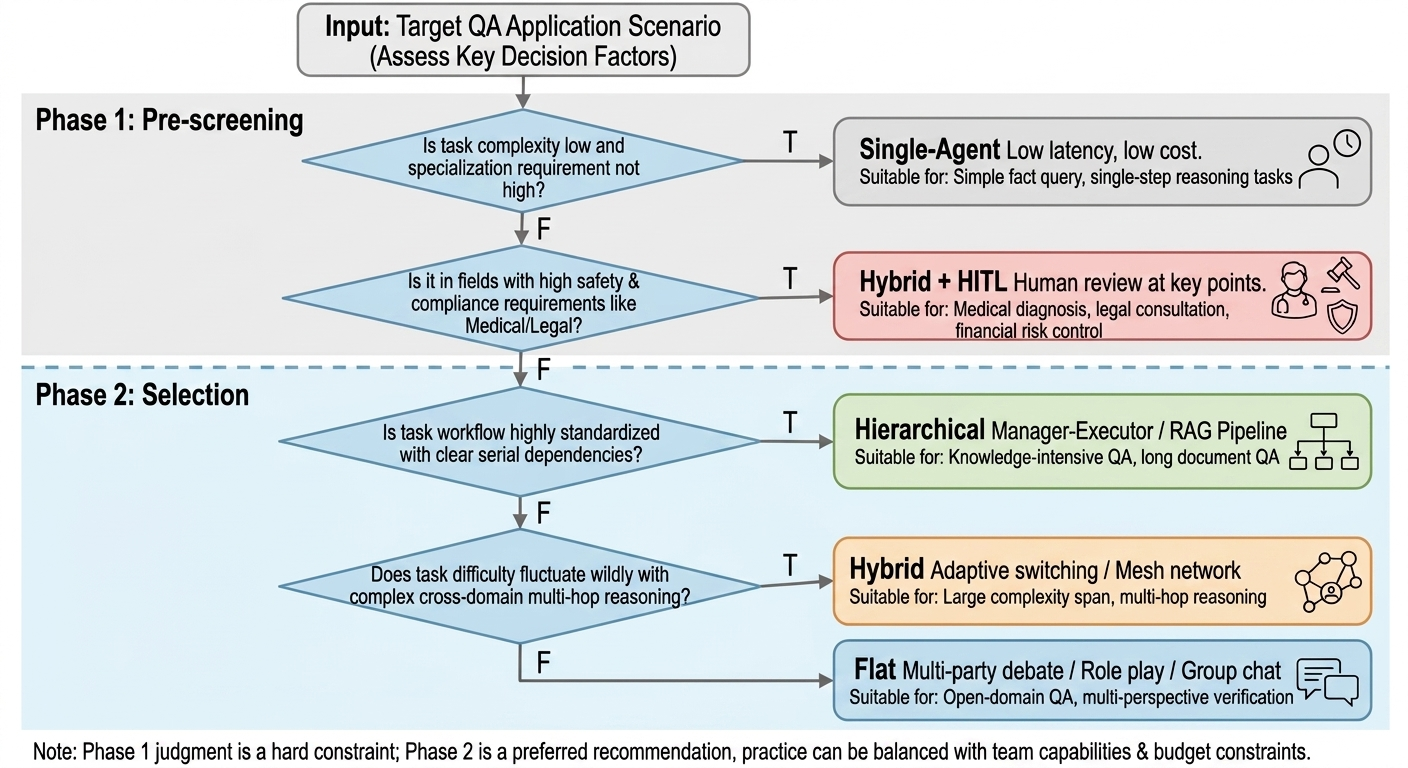
\includegraphics[width=0.80\linewidth]{fig_flow.jpg}
  \caption{Two-phase decision flowchart for multi-agent QA architecture
           selection across application scenarios.}
  \label{fig:decision_flow}
\end{figure*}

\subsubsection{Verification and illustrative applications}
\label{sec:case_studies}
\label{sec:validation}

The approach is verified for interpretive consistency by comparing its
inferred architectures with ten published systems. This purposive sample was
selected because the systems report agent roles and control flow with enough
detail for coding and cover different domains, process structures, and risk
levels. The comparison does not evaluate system performance, establish causal
benefit, or claim external validity.

Five cases are broadly aligned, three are partially aligned, and two are
divergent under the coding used here. MedAgents and LLM-MedQA combine
parallel expert perspectives with staged synthesis; MAD is flat at the macro
level but uses iterative convergence; EduPlanner and Financial Reflection QA
combine convergent objectives with evaluator or critic feedback. These boundary
cases show that competing requirements can make a single categorical label
insufficient and that a multi-label description of control flow may sometimes
be preferable.

\begin{table*}[pos=t]
  \centering
  \caption{Diagnostic comparison of the architecture-selection approach with ten published systems.}
  \label{tab:validation}
  \small
  \begin{tabularx}{\textwidth}{p{3.0cm} X p{3.0cm} c}
    \toprule
    \textbf{System} & \textbf{Application and criterion profile} &
    \textbf{Inferred versus source-based architecture coding} & \textbf{Match} \\
    \midrule
    MedAgents \citep{tang2024medagents} & Multi-specialty medical QA; high complexity and moderate risk & Flat versus hybrid staged synthesis & $\triangle$ \\
    LLM-MedQA \citep{tang2025llmmedqa} & Standardised medical MCQ; convergent objective with diverse views & Flat versus hybrid voting pipeline & $\triangle$ \\
    LegalGraphRAG \citep{legalgraphrag2026} & Legal verdict prediction; high risk and structured retrieval & Hybrid versus hybrid graph audit chain & $\checkmark$ \\
    Triad \citep{hu2024triad} & Knowledge-base QA; standardised Text-to-SPARQL workflow & Hierarchical versus hierarchical pipeline & $\checkmark$ \\
    LONGAGENT \citep{zhao2024longagent} & Ultra-long multi-hop QA; divide-and-conquer process & Hierarchical versus hierarchical leader--member workflow & $\checkmark$ \\
    ChatDev \citep{qian2023chatdev} & Software engineering; highly standardised stages & Hierarchical versus hierarchical ChatChain & $\checkmark$ \\
    AgentCoder \citep{huang2023agentcoder} & Code generation; explicit three-role dependencies & Hierarchical versus hierarchical feedback loop & $\checkmark$ \\
    MAD \citep{du2024multiagent_debate} & Open-domain reasoning; open process and low risk & Flat versus flat iterative convergence & $\triangle$ \\
    EduPlanner \citep{zhang2024eduplanner} & Educational planning; open and convergent requirements & Flat versus hierarchical evaluator--optimizer & $\times$ \\
    Financial Reflection QA \citep{fatemi2024financialqa} & Numerical QA; convergence with critic feedback & Hierarchical versus hybrid reflection loop & $\times$ \\
    \bottomrule
  \end{tabularx}
  \footnotesize
  \textit{Note}: $\checkmark$ = broadly aligned; $\triangle$ = partially aligned;
  $\times$ = divergent. Both architecture labels are the authors' coding of
  the selection approach and the reported workflow, not independent validation.
  Triad uses one LLM in three roles and is retained as an eligibility boundary case.
\end{table*}

The criteria can also be applied analytically to contrasting settings. In
high-risk, cross-domain consultation, parallel specialist analysis may improve
coverage, but final decisions require an explicit review boundary, making a
hybrid workflow with human approval a plausible candidate. Standardised,
evidence-grounded QA generally supports a hierarchical RAG baseline with
source and citation checks. Open-ended educational or legal tasks may benefit
from bounded peer critique, but legal use additionally requires auditability
and human accountability. These examples illustrate how task and governance
requirements constrain the design space; they do not imply one universally
correct topology.

\subsubsection{Summary and limitations}
\label{sec:limitations}

The approach makes architecture selection explicit through four criteria, a
two-phase flowchart, illustrative cases, and a diagnostic comparison with ten
published systems. Its limitations are substantial: competing requirements
can make a single topology label inadequate; the framework and model ecosystem
change rapidly; the purposive sample cannot establish external validity; and
the criteria remain qualitative rather than calibrated on a large labelled
system corpus. Independent coders, larger preregistered samples, quantitative
cost and quality measures, and prospective comparisons with alternative
selection procedures are needed.

% ==============================================================================
% SECTION 4: KEY TECHNOLOGIES IN MULTI-AGENT COLLABORATIVE QA
% ==============================================================================
\section{Key technologies in multi-agent collaborative QA}
\label{sec:key_tech}

The efficient operation of a multi-agent collaborative QA system depends not only on a well-designed organizational architecture but also on the support of core underlying technologies.
This section investigates five technological dimensions: communication
mechanisms, task decomposition, memory management, knowledge management, and
reasoning mechanisms.

% ── 4.1  Communication Mechanisms ─────────────────────────────────────────────
\subsection{Agent communication mechanisms}
\label{sec:comm}

Agent communication mechanisms determine how information is exchanged among
agents during collaborative QA. They support the transfer of queries,
intermediate findings, evidence, and feedback, and thereby shape coordination,
traceability, and communication cost. Communication may occur through direct
messages or through changes to a shared environment; interoperability
protocols provide a related interface for connecting agents with tools and
data sources. The following subsections distinguish these interaction
mechanisms from the protocols that support cross-system communication.

\subsubsection{Explicit communication}
\label{sec:explicit_comm}

Explicit communication refers to the direct transfer of information between agents via predefined formats.
The most common form is message passing based on structured languages (JSON,
XML) or dedicated prompt templates.
For example, AutoGen \citep{wu2024autogen} provides a representative implementation:
customisable conversable agents send and receive natural-language or code
messages following conversation patterns defined by developers.
ChatDev \citep{qian2023chatdev} provides another example by organising role-specialised agents
through a multi-turn dialogue chain covering design, coding, and testing stages.


\subsubsection{Implicit communication}
\label{sec:implicit_comm}

Implicit communication does not require direct agent-to-agent messaging; instead, collaboration is mediated via modifications to a shared operating environment.
For instance, in a code-generation QA task, one agent alters the state of a code repository or database, while another agent obtains feedback by observing compilation errors or test execution results.

This paradigm can reduce redundant message transfers, though its impact on communication overhead and fault tolerance is contingent on the implementation and task environment.

\subsubsection{Standardised communication protocols}
\label{sec:protocols}
Industry initiatives address different parts of the interface problem.
Anthropic introduced the Model Context Protocol (MCP)
\citep{anthropic2024mcp} to standardise connections to external tools and data
sources. Google's Agent2Agent (A2A) protocol \citep{google2025a2a} supports
communication and task coordination between agents across frameworks and
vendors. These interfaces can support heterogeneous multi-agent QA systems.

Explicit messaging makes the content and
provenance of an agent's contribution inspectable, and is useful when agents
must exchange evidence, explain decisions, or coordinate across distinct
roles. Its main cost is message volume: repeated dialogue consumes context
and adds latency, particularly as the team grows. Implicit communication
reduces direct message passing by using shared environmental state, but it
depends on agents being able to observe and interpret that state consistently;
otherwise, changes may be ambiguous or difficult to audit. Standardized
protocols address a different problem. MCP and A2A aim to improve
interoperability between tools, data sources, and agents, but protocol
compatibility alone does not guarantee useful coordination or reliable QA.
Thus, explicit and implicit communication are interaction mechanisms,
whereas protocols provide an interface layer that may support either.
Selection should reflect the need for traceability, the availability of
shared state, and the expected interaction cost
\citep{wu2024autogen,qian2023chatdev,anthropic2024mcp,google2025a2a}.

% ── 4.2  Task Decomposition and Scheduling ────────────────────────────────────
\subsection{Task decomposition and scheduling}
\label{sec:task_decomp}

Task decomposition and scheduling determine how a complex QA query is divided
into manageable work and how that work is assigned and coordinated. Their
purpose is to make interdependent reasoning steps tractable, enable
specialisation or parallel execution where appropriate, and ensure that
sub-results can be combined into a coherent answer. The discussion proceeds
from decomposing a query, to assigning subtasks to suitable agents, and then
to optimising or adapting their execution.

\subsubsection{Hierarchical task decomposition}
\label{sec:hier_decomp}

For complex QA tasks, LLMs often cannot answer in a single step.
Hierarchical task decomposition reduces difficulty by breaking complex queries
into sub-tasks that can be processed in parallel or sequentially.
Representative methods include Least-to-Most Prompting
\citep{zhou2023least_to_most} and Decomposed Prompting
\citep{khot2023decomposed_prompting}, which allow a model to solve simpler
sub-problems first and then exploit their answers to resolve the ultimate
target. Plan-and-Solve \citep{wang2023plan_and_solve} provides another example
by explicitly separating planning from solving and reducing missing-step
errors on the evaluated reasoning tasks.
Formally, given a complex query $Q$, a decomposition function $\mathcal{D}$
maps it to an ordered sequence of sub-tasks:
\begin{equation}
  \begin{aligned}
    \mathcal{D}(Q) &\to \{q_1, q_2, \ldots, q_m\}, \\
    \operatorname{Answer}(Q) &=
    \mathcal{F}\!\left(\operatorname{Sol}(q_1),\ldots,\operatorname{Sol}(q_m)\right)
  \end{aligned}
  \label{eq:decompose}
\end{equation}
where $\operatorname{Sol}(q_i)$ is a sub-agent's solution to sub-task $q_i$
and $\mathcal{F}$ is an aggregation function (e.g., voting, concatenation, or
re-generation).

\subsubsection{Role-based task assignment}
\label{sec:role_assign}

After decomposition, the system must assign sub-tasks to suitable agents.
For example, MetaGPT \citep{hong2024metagpt} organises agents through
predefined software-engineering roles, while AgentVerse
\citep{chen2024agentverse} recruits experts by generating task-specific
expertise descriptions and adjusts team composition using evaluation
feedback. These mechanisms guide which agents contribute to a task;
their scheduling efficiency requires separate evaluation.

\subsubsection{Pipeline optimisation and adaptive orchestration}
\label{sec:load_balance}

Static assignment can be inefficient when task difficulty and agent capabilities vary across queries. For example, DSPy \citep{khattab2024dspy} addresses a related but narrower problem: it represents language-model pipelines as declarative modules and compiles their prompts and demonstrations against a task metric. It should therefore be regarded as a pipeline-optimization toolkit rather than evidence supporting runtime multi-agent load balancing. Dynamic agent recruitment, routing, and early stopping remain distinct orchestration decisions that require task-specific evaluation.

Decomposition, assignment, and orchestration
solve related but distinct problems. Decomposition determines which
sub-questions must be answered and how they depend on one another; assignment
matches those sub-questions to agents; orchestration determines their
execution order and whether the workflow should adapt at runtime.
Least-to-Most, Decomposed Prompting, and Plan-and-Solve primarily inform the
first decision, whereas role profiles in MetaGPT and AgentVerse address the
second \citep{zhou2023least_to_most,khot2023decomposed_prompting,
wang2023plan_and_solve,hong2024metagpt,chen2024agentverse}. A fixed sequence
is adequate when dependencies and agent capabilities are known in advance;
dynamic routing may be more suitable when query difficulty or available
expertise varies, but it adds scheduling overhead and failure points. In
either case, decomposition errors can propagate: omitted sub-questions leave
gaps in the final answer, while unnecessary decomposition creates redundant
calls and aggregation work. Pipeline-optimization tools such as DSPy can
improve task-metric performance of language-model modules, but should not be
treated as evidence that runtime recruitment or load balancing is effective
\citep{khattab2024dspy}. Evaluation should distinguish decomposition quality,
assignment fit, and orchestration efficiency rather than attributing an
end-to-end gain to a single mechanism.

% ── 4.3  Knowledge Management ────────────────────────────────────────────────
\subsection{Knowledge management}
\label{sec:knowledge_management}

Knowledge management concerns how external, retrieved, and agent-generated
information is represented, validated, and made available to the team. It
provides a shared evidence basis for collaborative QA and aims to reduce
duplicated information seeking without allowing unverified content to spread.
It is therefore a system-level layer built on, but not equivalent to,
individual agent memory.

In complex collaboration, knowledge must not be siloed within individual
agents.
The system needs a global knowledge graph shared across agents so that all
collaborative nodes can synchronise critical facts in real time.
By constructing a shared graph-vector database, newly spawned sub-agents
can rapidly inherit the team's cumulative knowledge, avoiding redundant
retrieval and cognitive divergence.

Knowledge management operates above individual
memory. A shared graph or vector store can provide a common evidence base and
reduce duplicated retrieval, but unrestricted sharing can also spread stale,
irrelevant, or erroneous content across the team. Practical designs should
attach provenance, timestamps, confidence, and validation status to shared
facts, and should allow agents to revise or withdraw them. The key design
questions are which knowledge is shared, which agents may access it, how
conflicts are resolved, and how retrieved or generated content is verified
before it becomes reusable team knowledge.

% ── 4.4  Memory Management ───────────────────────────────────────────────────
\subsection{Memory management}
\label{sec:memory}

Memory management concerns the information state retained by an agent or
workflow over time. It preserves relevant context across interaction turns and
supports continuity when a task spans multiple reasoning steps. It is distinct
from knowledge management: memory concerns retention and recall of state,
whereas knowledge management concerns the organisation, validation, and
distribution of reusable information.

\subsubsection{Short-term memory and working memory}
\label{sec:short_mem}

Short-term memory preserves dialogue history and local context for the
current QA session. For example, MemGPT \citep{packer2023memgpt} draws on
operating-system memory hierarchies to manage a limited main context and
external memory. Function calls control information transfer between them,
while a FIFO message queue and recursive summaries manage dialogue context
under the context-window limit.

\subsubsection{Long-term memory and vector retrieval (RAG)}
\label{sec:long_mem}

Long-term memory can retain historical experiences and domain knowledge in
external stores \citep{zhang2024memory_survey}. Vector retrieval is one way
to access such information: Retrieval-Augmented Generation (RAG)
\citep{lewis2020rag,gao2024rag_survey} augments generation with retrieved
documents. As one illustrative multi-agent implementation, a retrieval agent
can select the Top-$k$ relevant documents from knowledge base $\mathcal{D}$
using cosine similarity:
\begin{equation}
  \operatorname{Rel}(q,d_i) =
  \frac{\boldsymbol{\phi}(q)^{\top}\boldsymbol{\phi}(d_i)}
       {\|\boldsymbol{\phi}(q)\|\,\|\boldsymbol{\phi}(d_i)\|},\qquad
  \hat{\mathcal{D}} =
  \operatorname*{Top\text{-}k}_{d_i\in\mathcal{D}}\operatorname{Rel}(q,d_i)
  \label{eq:rag}
\end{equation}
where $\boldsymbol{\phi}(\cdot)$ is the dense encoder embedding function and
$\hat{\mathcal{D}}$ is the set of retrieved relevant documents. Retrieval has
evolved from passive retrieval to active variants. Self-RAG
\citep{asai2024selfrag} uses reflection tokens to decide when to retrieve and
to critique generated passages, while FLARE \citep{jiang2023active_rag}
triggers retrieval when predicted upcoming text contains low-confidence
tokens and then regenerates that text. These controls can inform retrieval
components in a multi-agent workflow.

Short-term and long-term memory address
different temporal scopes. Working memory supports continuity within the
current interaction and must prioritise information under a limited context
budget; long-term memory extends access beyond that context, but depends on
retrieval relevance and the quality and currency of stored experiences or
documents. MemGPT illustrates session-context management, whereas RAG and its
retrieval variants provide access to information outside the active context
\citep{packer2023memgpt,lewis2020rag,gao2024rag_survey,asai2024selfrag,
jiang2023active_rag}. A system should therefore specify what is retained, for
how long, and under what conditions memories are updated or discarded.

% ── 4.5  Reasoning Mechanisms ─────────────────────────────────────────────────
\subsection{Reasoning mechanisms}
\label{sec:reasoning}

Reasoning mechanisms aim to improve answer quality by broadening
the available reasoning paths, distributing evidence processing, or revisiting
provisional conclusions to detect errors. In collaborative QA, these methods
can complement one another, but they target different constraints and may add
inference cost. The following categories cover collaborative reasoning and
answer aggregation, reasoning distributed across agents, and reflection or
critique of generated answers.

\subsubsection{Collaborative chain-of-thought}
\label{sec:cot}

Chain-of-Thought (CoT) prompting \citep{wei2022chain_of_thought}
can improve performance on evaluated arithmetic, commonsense, and symbolic
reasoning tasks.
Self-Consistency \citep{wang2023self_consistency} provides a representative
single-model method: it samples multiple reasoning paths and selects an answer
by marginalising over those paths. Multi-agent systems adapt this diversity
principle by assigning independent
reasoners and then using debate or confidence-aware aggregation
\citep{du2024multiagent_debate,chen2024reconcile}.

In the single-model baseline, $K$ reasoning paths
$\{(r_k, a_k)\}_{k=1}^{K}$ are sampled for the same question, and majority
voting selects the final answer:
\begin{equation}
  \hat{a} = \underset{a\in\mathcal{Y}}{\arg\max}\sum_{k=1}^{K}
  \mathbf{1}\!\left[f_\theta(x,r_k)=a\right]
  \label{eq:self_consistency}
\end{equation}
where $f_\theta(x,r_k)$ is the answer produced by the $k$-th reasoning
chain and $\mathbf{1}[\cdot]$ is the indicator function.
The equation describes the single-model Self-Consistency baseline; exchange
between agents is an additional collaboration design, not a property of the
original method.

\subsubsection{Chain-of-agents reasoning}
\label{sec:chain_of_agents}

For ultra-long-text QA, the attention mechanism of conventional
Transformers faces severe computational bottlenecks.
Chain-of-Agents \citep{zhang2024chain_agents} distributes evidence processing
across worker agents, while Tree of Thoughts
\citep{yao2023tree_of_thoughts} and Graph of Thoughts
\citep{besta2024graph_of_thoughts} organise intermediate reasoning states as
search structures.
In Chain-of-Agents, worker agents process successive text chunks and pass
forward condensed evidence before a manager produces the answer. LONGAGENT
\citep{zhao2024longagent} uses a different leader--member design in which a
leader coordinates member agents over long-document segments. Tree- and
graph-structured reasoning provide related search topologies, but are not
necessarily multi-agent systems in their original formulations.

\subsubsection{Self-reflection and mutual-critique mechanisms}
\label{sec:reflexion}

To suppress hallucination, agents must be capable of iterative
self-examination.
For example, Reflexion \citep{shinn2023reflexion} stores linguistic feedback
from prior trials in episodic memory, whereas Self-Refine
\citep{madaan2023self_refine} provides another example by iterating between generation, feedback, and
revision without additional model training.
Chain-of-Verification \citep{dhuliawala2023chain_of_verification} drafts an
answer, plans verification questions, answers them independently, and then
revises the original answer. This procedure targets factual errors; dedicated
critic agents are a possible multi-agent extension that requires evaluation.

These techniques seek reliability through
different mechanisms. Self-consistency and debate broaden the set of candidate
reasoning paths; Chain-of-Agents distributes evidence processing across long
inputs; reflection and critique revisit a provisional answer to identify and
repair errors \citep{wang2023self_consistency,du2024multiagent_debate,
zhang2024chain_agents,shinn2023reflexion,madaan2023self_refine,
dhuliawala2023chain_of_verification}. They are not interchangeable: sampling
more paths helps only when those paths provide meaningful diversity,
sequential evidence transfer can lose information, and a critic may share the
generator's blind spots. Combining mechanisms is possible, but each extra
pass adds inference cost and requires an aggregation or stopping rule. The
appropriate choice therefore depends on the dominant failure mode: ambiguity
among plausible answers, limited capacity to process long evidence, or the
need to audit a provisional response. Reliability should be evaluated against
these failure modes rather than inferred from the number of agents or
reasoning rounds.

% ==============================================================================
\iffalse
% LEGACY APPLICATION-DOMAIN SECTION AND STANDALONE SELECTION GUIDE
% SECTION 5: TYPICAL APPLICATION DOMAINS
% ==============================================================================
\section{Application domains and task-specific architecture requirements}
\label{sec:applications}

The value of multi-agent collaboration depends on the structure and
governance requirements of the target application, rather than on the domain
label alone. This section therefore examines representative application
domains through four common questions: what makes the QA task difficult, which
roles or control patterns are used, what evidence is available, and what
constraints limit deployment. The domains were selected to cover different
combinations of specialized knowledge, evidence requirements, interaction
patterns, and risk. Table~\ref{tab:app_compare} provides an analytical
overview of the principal examples; it is not a ranking of application
performance, and the representative systems do not all carry the same
evidentiary status in the review.

\begin{table*}[pos=t]
  \centering
  \caption{Comparison of typical applications of multi-agent collaborative QA systems.}
  \label{tab:app_compare}
  \scriptsize
  \setlength{\tabcolsep}{3pt}
  \begin{tabular}{p{1.8cm} p{2.4cm} p{4.0cm} p{4.0cm} p{4.0cm}}
    \toprule
    \textbf{Domain} & \textbf{Representative System} &
    \textbf{Core Challenge} & \textbf{Collaboration Pattern} &
    \textbf{Performance Highlights} \\
    \midrule
    Healthcare &
      MedAgents \citep{tang2024medagents} &
      Extremely high factual accuracy demands; long-tail rare-disease diagnosis &
      Multi-specialty physician role-play; symptom--pathology cross-verification &
      Improves zero-shot medical reasoning across nine evaluated datasets \\[6pt]
    Legal &
      ChatLaw \citep{cui2023chatlaw} &
      Retrieval from voluminous legal statutes; rigorous formal-logic reasoning &
      Plan--Retrieve--Generate pipeline; statute-matching and verdict-prediction agents collaborate &
      More rigorous responses to long case texts on LegalBench \\[6pt]
    Education &
      GenMentor \citep{li2024genmentor} &
      Heuristic guidance rather than direct answers; personalized adaptation &
      Tutor, encourager, and evaluator roles in a mixed-role network &
      Multi-path learning recommendations; interaction closer to a human private tutor \\[6pt]
    Enterprise support &
      Generative-AI assistant \citep{brynjolfsson2023generative_ai_work} &
      Integration with corporate knowledge and back-end service workflows &
      Retrieval, service triage, and ticket or action execution can be assigned to specialized components &
      Adjacent deployment evidence; reports increased issue resolution per hour \\[6pt]
    Software Engineering &
      ChatDev \citep{qian2023chatdev} &
      Cross-file logic dependencies; multi-round compilation and debug feedback &
      SOP-based waterfall; product, development, and testing roles in group-chat collaboration &
      Full closed-loop of automated writing, reviewing, and running code \\
    \bottomrule
  \end{tabular}
\end{table*}

The following subsections first discuss the domain-specific cases and then
extract requirements that cut across domains. This order separates the
descriptive question of where collaborative QA is used from the comparative
question of which architectural properties those settings require.

\subsection{Medical QA}
\label{sec:medical}

The medical domain imposes extremely high standards of factual accuracy
and rigour.
For example, MedAgents \citep{tang2024medagents} proposes a multi-disciplinary
cross-verification collaborative framework that simulates a multi-specialty
expert consultation, effectively addressing the deficiencies of single-model
reasoning on complex rare-disease cases.
MDAgents \citep{kim2024mdagents} provides another example by adaptively assigning solo or group
collaboration according to estimated case complexity. Med-PaLM
\citep{singhal2023medpalm}, by contrast, is a domain-specialized medical LLM
rather than a multi-agent system; it is relevant as a possible expert backbone,
not as evidence that adaptive agent recruitment itself reduces clinical risk.

\subsection{Legal QA}
\label{sec:legal}

Legal case QA typically involves precise retrieval over voluminous case
files and statutes.
For Chinese-language legal domains, ChatLaw \citep{cui2023chatlaw} provides an example that
integrates an external legal knowledge base and employs RAG for multi-hop
retrieval.
LegalBench \citep{guha2023legalbench} is a general legal-reasoning benchmark,
not evidence for a particular multi-agent topology. A directly relevant
example is LegalGraphRAG \citep{legalgraphrag2026}, which separates evidence
retrieval, source auditing, and adjudication in a graph-grounded pipeline.
This design makes evidence provenance more explicit, although benchmark
performance does not by itself establish suitability for autonomous legal use.

\subsection{Educational QA}
\label{sec:education}

In intelligent education settings, QA systems should not merely provide
correct answers; they should guide students to think independently.
For example, the GenMentor framework \citep{li2024genmentor} introduces multiple roles
including tutor, corrector, and knowledge extender to construct
goal-oriented personalized learning paths.
Agents collaboratively adjust the depth of explanation in real time
based on student feedback, realizing Socratic heuristic teaching.

\subsection{Customer service and office automation}
\label{sec:enterprise}

In enterprise customer service and process automation, multi-agent QA
systems can directly integrate with back-end corporate APIs.
For example, empirical research by \citet{brynjolfsson2023generative_ai_work}
reports a 15\% average increase in issues resolved per hour in one firm's
deployment of a generative-AI assistant.
By delegating knowledge retrieval, sentiment management, and ticket creation
to dedicated sub-agents, the system achieves 24-hour unattended, efficient
problem resolution and fault diagnosis.

\subsection{Code generation and technical QA}
\label{sec:code}

Code generation is one of the most mature application areas for multi-agent
systems.
For example, SWE-agent \citep{yang2024swe_agent} and ChatDev \citep{qian2023chatdev}
convert complex software-engineering requirements into multi-round
collaborative workflows.
On the SWE-bench benchmark \citep{jimenez2024swe_bench}, collaborative
pipelines in which an architect agent generates the framework, a programmer
agent writes the code, and a testing agent provides compilation feedback
not only answer programming questions but directly generate complete
multi-thousand-line projects.

\subsection{Cross-domain architecture requirements}
\label{sec:application_requirements}

The applications reviewed above differ less in their use of multiple agents
than in the requirements that make coordination useful. Medical and legal QA
combine broad domain knowledge with strong provenance and accountability
requirements; they therefore favor evidence-grounded workflows with explicit
review boundaries. Enterprise knowledge-base QA and long-document QA are more
highly standardized: retrieval, synthesis, and verification can often be
organized as a controlled pipeline, provided that evidence transfer and source
access are audit-able. Educational and open-domain QA place greater emphasis on
explanation, adaptation, and alternative perspectives, making moderated peer
interaction potentially useful. Software engineering and other tool-mediated
tasks have explicit artifacts and executable feedback, which support staged
delegation and iterative verification.

These observations provide the empirical basis for the selection framework in
Section~6. They suggest three cross-domain questions: how many dependent
reasoning steps and specialized knowledge sources are required; whether the
workflow is stable or must adapt to the query and intermediate evidence; and
what level of error tolerance, provenance, and human accountability applies.
The application cases do not imply that a domain has one universally correct
architecture. Rather, they show how task and governance requirements constrain
the plausible design space and why the same architecture may be appropriate
in one setting but excessive or unsafe in another.
% ==============================================================================
% SECTION 6: ARCHITECTURE-SELECTION GUIDE FOR MULTI-AGENT QA
% ==============================================================================
\section{A framework for selecting multi-agent QA architectures}
\label{sec:guideline}

The preceding sections establish a descriptive taxonomy of multi-agent QA
architectures (Section~3), review the mechanisms that support them
(Section~4), and identify domain-specific requirements (Section~5). The
question addressed here is different: given a task, when is a single-agent,
flat, hierarchical, or hybrid workflow a defensible design choice? Additional
agents are not an unconditional improvement. They introduce communication,
aggregation, and failure-management costs, and may reduce performance when a
task does not benefit from decomposition or independent verification. The
MAST taxonomy likewise documents recurrent failures in system design,
inter-agent alignment, and task verification \citep{han2024mast}. This section
therefore turns the preceding evidence into a qualitative selection framework.
It is intended to make architectural reasoning explicit, not to replace
task-specific benchmark or safety validation.

% ── 6.1  Framework Scope and Purpose ──────────────────────────────────────────
\subsection{Framework scope and purpose}
\label{sec:framework_scope}

The framework treats the single-agent workflow as a valid baseline and uses
the three collaborative classes from Section~3 as candidate control patterns.
It links an application's task complexity, process structure, risk, and
auditability requirements to a plausible architecture and to the controls
that should accompany it. The output is therefore a reasoned shortlist rather
than a universal assignment: a candidate architecture must still be compared
with alternatives using task quality, latency, cost, provenance, and recovery
measures. This distinction prevents the taxonomy from being read as a claim
that multi-agent collaboration is preferable for every QA problem.

% ── 6.2  Architecture-selection criteria ─────────────────────────────────────
\subsection{Architecture-selection criteria}
\label{sec:decision_factors}

The framework uses four qualitative criteria to assess whether an
architecture is appropriate for a given QA task. Together, they describe the
task properties, operational constraints, and governance requirements that
make an architecture choice defensible. They support comparison across
heterogeneous studies, but do not imply a universal numerical threshold or
claim that one architecture dominates the others.

\textbf{1.\ Task complexity and domain span.} The analysis starts
from the task's reasoning structure, evidence requirements, output criteria,
and domain span rather than from a preferred framework or model family. The
complexity criterion captures the number and interdependence of reasoning
steps, the breadth of required expertise, and the need for independent
evidence sources. Single-agent execution is often adequate for short,
low-uncertainty queries. Decomposition and role specialization become more
plausible when a task combines separable sub-tasks or domains, such as
multi-specialty consultation or a software-engineering loop. Complexity alone,
however, does not establish that multiple agents will improve the answer; the
additional roles must contribute distinct information or checks.

\textbf{2.\ Process standardization and dynamism.} This criterion concerns
whether the workflow has stable stages and dependencies or must adapt to
evidence and query state. Explicit dependencies favor hierarchical or
pipeline control, whereas open-ended tasks may benefit from peer generation
and critique. When the appropriate mode changes across queries or stages,
hybrid routing is a candidate design. These are tendencies rather than
deterministic mappings: a hierarchical workflow can contain local debate, and
a flat workflow can still enforce turn limits and aggregation rules.

\textbf{3.\ Cost and resource burden.} Multi-agent execution generally adds
communication, aggregation, state-management, and inference costs. A
collaborative design is justified only when the expected improvement in
coverage, reliability, or adaptability is large enough to offset those costs
\citep{han2024mast}. Cost should therefore be assessed together with latency,
token use, tool calls, and the operational burden of monitoring and recovery.

\textbf{4.\ Risk tolerance and auditability.} This risk-sensitive criterion
determines how much decision authority can be delegated and what evidence must
be retained. Low-risk exploratory tasks may tolerate approximate answers,
whereas healthcare, legal, financial, and other consequential applications
require provenance, review, contestability, and explicit responsibility for
final decisions. Human-in-the-loop checkpoints are one possible control, but
their placement and scope depend on the domain, the type of decision, and the
applicable governance requirements; their effectiveness must be evaluated
rather than assumed.

% ── 6.3  Two-Phase Decision Flow ──────────────────────────────────────────────
\subsection{Two-phase architecture-selection procedure}
\label{sec:two_phase}

The four criteria are combined in the two-phase flow shown in
Fig.~\ref{fig:decision_flow}. The flow is a screening heuristic: it narrows
the set of plausible designs and makes trade-offs explicit, but it does not
replace empirical comparison of candidate implementations.

The flow is developed as a design artifact following the Design Science
Research Methodology (DSRM) \citep{peffers2007dsrm}. In this application,
problem identification and objective definition motivate the need for a
transparent selection procedure; design and development translate the
architecture, technology, and application review into the four selection
criteria; demonstration uses contrasting QA scenarios; and verification
compares the framework's interpretations with ten published systems rather
than claiming external validation. The procedure is therefore a structured design
proposal whose assumptions and limitations remain open to empirical testing.

\textbf{Phase 1 (pre-screening).} First establish whether the task can be
handled by one workflow at the required quality and cost. If so, a single-agent
baseline remains a valid candidate. If the task requires separable expertise,
long-horizon reasoning, or independent verification, multi-agent designs are
retained for the second phase. Risk and auditability are then used to constrain
the permissible degree of autonomy; in consequential settings, this may imply
human review or other external controls, but not necessarily one fixed
topology.

\textbf{Phase 2 (topology selection).} For the remaining candidates, compare
the process structure and information dependencies. Stable stages and explicit
hand-offs support hierarchical control; peer generation and critique support
flat collaboration when independent perspectives are valuable; changing
requirements or conditional review support hybrid control. The selected design
should then be compared with a single-agent baseline using task quality,
latency, cost, provenance, and failure-recovery measures.

\begin{figure*}[pos=t]
  \centering
  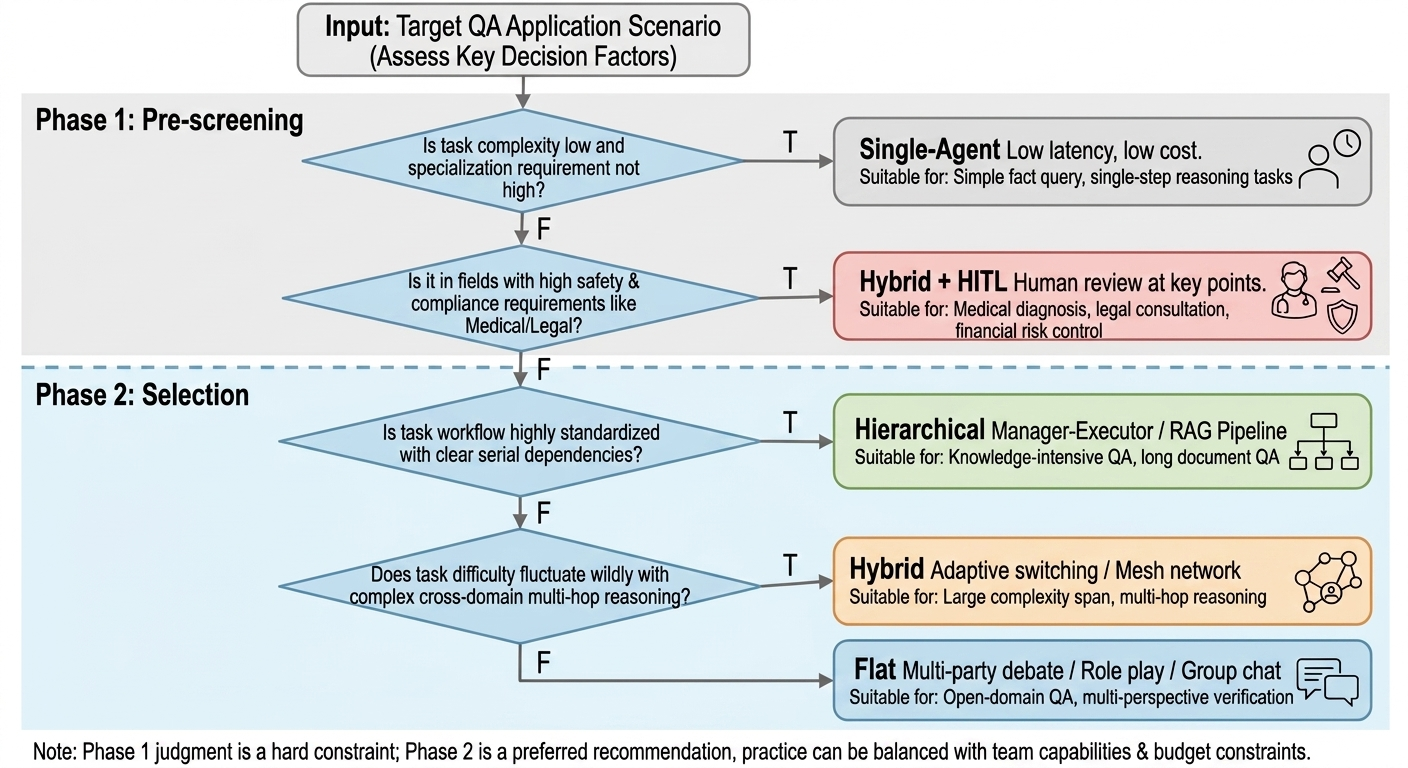
\includegraphics[width=0.80\linewidth]{fig_flow.jpg}
  \caption{Two-phase decision flowchart for multi-agent QA architecture
           selection across application scenarios.}
  \label{fig:decision_flow}
\end{figure*}

\clearpage
\onecolumn
% ── 6.4  Verification of the Selection Framework ──────────────────────────────
\subsection{Verification of the selection framework}
\label{sec:case_studies}
\label{sec:validation}

This section verifies the framework's interpretive consistency by comparing
its inferred architectures with those reported for published systems and by
applying its criteria to contrasting QA scenarios. This verification does not
evaluate system performance, establish causal benefit, or claim external
validity. For the system comparison, the framework is applied to ten published
systems using a deduction--comparison procedure. The
sample is purposive rather than random. Cases were included when their
publication fell within the survey window, their agent roles and control flow
were described sufficiently for coding, and they contributed variation in
domain, process structure, and risk. The sample covers healthcare, legal,
software engineering, education, finance, and general or enterprise QA. Each
case is coded on the four selection criteria, an architecture is inferred,
and the inference is compared with the architecture reported by the original
authors (Table~\ref{tab:validation}). The procedure evaluates interpretive
consistency; it does not estimate accuracy, causal benefit, or external
validity.

Five cases are broadly aligned, three are partially aligned, and two are
divergent under the coding used here. LegalGraphRAG, Triad, LONGAGENT,
ChatDev, and AgentCoder follow the inferred architecture closely. MedAgents
and LLM-MedQA combine parallel expert perspectives with staged synthesis, so
their implemented workflows are more hybrid than a flat label suggests. MAD
\citep{du2024multiagent_debate} is flat at the macro level but uses iterative
convergence rather than the explicit vote procedure anticipated by the guide.
EduPlanner \citep{zhang2024eduplanner} and Financial Reflection QA
\citep{fatemi2024financialqa} combine convergent objectives with evaluator or
critic feedback, producing divergent classifications. These boundary cases
indicate that task dimensions can conflict and that a single categorical label
may conceal meaningful control-flow differences. The counts should therefore
be read as author-coded diagnostic observations, not as a validation score.

\begin{center}
  \captionof{table}{Verification of the architecture-selection framework through comparison with 10 published systems.}
  \label{tab:validation}
  \small
  \resizebox{\linewidth}{!}{%
  \begin{tabular}{p{2.2cm} p{2.6cm} p{4.8cm} p{2.4cm} p{3.4cm} c}
    \toprule
    \textbf{System} & \textbf{Application} &
    \textbf{Key Decision-Factor Profile} &
    \textbf{Inferred Arch.} & \textbf{Actual Arch.} &
    \textbf{Match} \\
    \midrule
    MedAgents \citep{tang2024medagents} &
      Multi-specialty medical QA &
      Cross-specialty high complexity; non-standardisable reasoning; moderate risk &
      Flat (multi-role collaboration) &
      Hybrid (parallel expert analyses + staged synthesis and decision) & $\triangle$ \\[3pt]
    LLM-MedQA \citep{tang2025llmmedqa} &
      Standardised medical MCQ &
      Moderate complexity; convergent objective but divergent perspectives; moderate risk &
      Flat (multi-view + vote aggregation) &
      Hybrid (question/option experts + six-stage voting and decision pipeline) & $\triangle$ \\[3pt]
    LegalGraphRAG \citep{legalgraphrag2026} &
      Legal verdict prediction &
      Multi-level legal reasoning; standardize retrieval + open reasoning; zero-tolerance high risk &
      Hybrid (hierarchical RAG + flat review) &
      Hybrid (layered graph + three-role audit chain) & \checkmark \\[3pt]
    Triad \citep{hu2024triad} &
      Enterprise structured KBQA &
      Moderate complexity; Text-to-SPARQL highly standardised; moderate risk &
      Hierarchical (rigid pipeline) &
      Hierarchical (three-role four-stage serial pipeline) & \checkmark \\[3pt]
    LONGAGENT \citep{zhao2024longagent} &
      Ultra-long document multi-hop QA &
      High complexity; divide-and-conquer SOP; moderate risk &
      Hierarchical (Leader--Member) &
      Hierarchical (Leader dispatch + Member parallel) & \checkmark \\[3pt]
    ChatDev \citep{qian2023chatdev} &
      Full-cycle software engineering &
      High complexity; very high waterfall standardisation; moderate risk &
      Hierarchical (waterfall pipeline) &
      Hierarchical (multi-role Chat Chain serial pipeline) & \checkmark \\[3pt]
    AgentCoder \citep{huang2023agentcoder} &
      Code generation and iterative testing &
      Moderate complexity; clear three-role data-flow dependency; low risk &
      Hierarchical (rigid three-role pipeline) &
      Hierarchical (coder $\to$ test-designer $\to$ executor + feedback loop) & \checkmark \\[3pt]
    MAD \citep{du2024multiagent_debate} &
      Open-domain factual \& maths reasoning &
      High openness; no standard workflow; low risk &
      Flat (multi-view debate + vote convergence) &
      Flat (peer debate + iterative convergence, no explicit vote round) & $\triangle$ \\[3pt]
    EduPlanner \citep{zhang2024eduplanner} &
      Adaptive educational planning &
      Open education + convergent curriculum-scoring objective; dual features; low risk &
      Flat (multi-view discussion) &
      Hierarchical (Evaluator--Optimizer adversarial pipeline) & $\times$ \\[3pt]
    Financial Reflection QA \citep{fatemi2024financialqa} &
      Financial numerical reasoning QA &
      Convergent target + reasoning requires self-critique; dual features; moderate risk &
      Hierarchical (RAG pipeline) &
      Hybrid (Solver + multi-Critic reflection loop) & $\times$ \\
    \bottomrule
  \end{tabular}}
  \footnotesize
  \textit{Note}: \checkmark = broadly aligned; $\triangle$ = partially
  aligned but with an additional coordination layer or different convergence
  mechanism; $\times$ = divergent inferred and implemented architecture.
  The labels are author coding and do not constitute independent validation.
\end{center}

The comparison is most informative where the criteria point in the same
direction and least decisive where requirements conflict. Such cases may
require explicit priority weights, cost constraints, or a multi-label
description of control flow. Larger samples, independent coders, and
prospective comparisons against alternative selection procedures would be
needed before stronger claims could be made.

The following examples illustrate how the criteria narrow the plausible
design space in specific application scenarios. They are analytical
illustrations rather than deployment prescriptions or comparative
performance claims.

\par\noindent\textbf{High-risk, cross-domain consultation.}
Medical consultation combines broad specialist knowledge with a low tolerance
for unsupported recommendations. Parallel retrieval or expert analysis may
improve coverage, but final triage or treatment decisions require an explicit
review boundary. A hybrid workflow with clinician approval is therefore a
plausible candidate. MDAgents \citep{kim2024mdagents} is a relevant
multi-specialty precedent, but does not establish the safety of any particular
deployment.

\par\noindent\textbf{Standardised, evidence-grounded QA.}
Enterprise policy QA and long-document QA generally require traceable sources
and a stable sequence of planning, retrieval, synthesis, and verification. A
hierarchical RAG pipeline is consequently a reasonable baseline, as illustrated
by LONGAGENT \citep{zhao2024longagent}. The design still requires access
controls, citation checking, and comparison with a simpler retrieval baseline.

\par\noindent\textbf{Open-ended tasks with competing requirements.}
Legal consultation and educational QA illustrate a different boundary. Both
may benefit from alternative interpretations or explanations, but legal use
also requires auditability and human accountability. A hybrid design can
combine controlled retrieval with bounded peer critique and domain-expert
review; in lower-risk educational settings, moderated peer interaction may be
sufficient. CAMEL and multi-agent debate provide relevant interaction
precedents \citep{li2023camel,du2024multiagent_debate}, not evidence that one
topology is universally optimal.

% ── 6.5  Summary and Limitations ──────────────────────────────────────────────
\subsection{Summary and limitations}
\label{sec:limitations}

This section has proposed a qualitative, task-driven procedure for comparing
single-agent and multi-agent architectures. Its contribution is to make the
reasoning behind a choice explicit through four selection criteria, a
two-phase flowchart (Fig.~\ref{fig:decision_flow}), illustrative cases, and a
verification against ten published systems. The procedure has three principal limitations. First,
competing requirements can make a single topology label inadequate. Second,
the rapidly changing framework and model ecosystem limits the temporal
stability of specific recommendations. Third, the purposive ten-case sample
cannot establish external validity. Future work should test the dimensions
with independent coders, larger and preregistered samples, quantitative cost
and quality measures, and prospective comparisons with alternative selection
methods.
\clearpage
\twocolumn
\fi
% ==============================================================================
% SECTION 5: DEVELOPMENT AND EVALUATION RESOURCES FOR MULTI-AGENT QA
% ==============================================================================
\section{Development and evaluation resources for multi-agent collaborative QA}
\label{sec:platform_benchmarks}

The preceding sections examined how multi-agent collaborative QA systems are
organized, implemented, selected, and applied. This section reviews the
resources needed to construct and assess such systems, following the four
layers shown in Fig.~\ref{fig:platform_resource_map}: foundation components,
multi-agent orchestration frameworks, application-oriented resources, and
benchmarks and evaluation tools. The layers serve complementary functions:
foundation components connect models and retrieval resources; orchestration
frameworks define agent roles and workflow control; application resources
instantiate task-oriented capabilities; and benchmarks and tools assess
answer quality and collaboration. The figure is a conceptual map, not a
requirement that every system use a single tool from each layer.

\begin{figure}[t]
	\centering
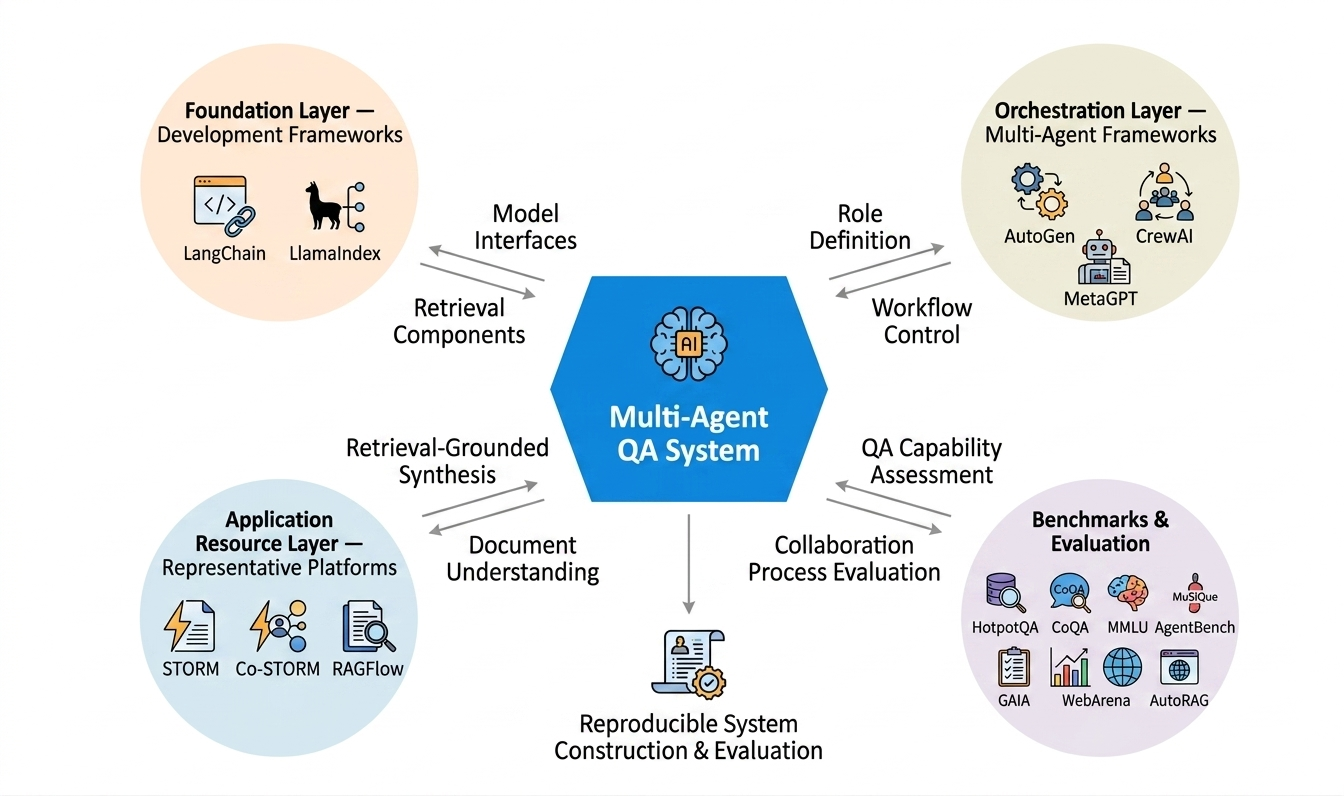
\includegraphics[width=\columnwidth]{classify.jpg}
\caption{Four resource layers for constructing and evaluating multi-agent collaborative QA systems.}
	\label{fig:platform_resource_map}
\end{figure}

% ── 7.1  Foundation Layer ────────────────────────────────────────────────────
\subsection{Foundation layer: model and retrieval components}
\label{sec:foundation_layer}

The foundation layer supplies the interfaces and reusable components on which
a QA workflow can be built. As illustrated in Fig.~\ref{fig:platform_resource_map},
development frameworks such as LangChain and LlamaIndex provide representative
model-interface and retrieval-component resources. At this layer, the main
concerns are connecting model services, preparing and retrieving evidence,
and making external data accessible to the system. These components support
retrieval-grounded answering, but do not by themselves assign responsibilities
to multiple agents or determine how their work is coordinated.

Interoperability protocols address part of this integration problem. For
example, the Model Context Protocol (MCP) standardizes connections between
models or agents and external tools and data sources \citep{anthropic2024mcp}.
Such interfaces can support several orchestration frameworks, but do not
specify role allocation, task decomposition, or decision authority. These
coordination functions belong to the orchestration layer discussed next.

% ── 7.2  Orchestration Layer ─────────────────────────────────────────────────
\subsection{Orchestration layer: multi-agent frameworks}
\label{sec:framework_compare}

The orchestration layer determines how agents are defined, assigned work, and
coordinated during execution. Figure~\ref{fig:platform_resource_map}
illustrates this layer with AutoGen, CrewAI, and MetaGPT
\citep{wu2024autogen,crewai2023,hong2024metagpt}. Across the wider set of
resources, some frameworks encode collaboration through predefined roles and
procedures: for example, CAMEL uses role-conditioned dialogue, while ChatDev
and MetaGPT organize work through staged, role-based processes
\citep{li2023camel,qian2023chatdev,hong2024metagpt}. Other frameworks expose
more control flow to developers: AutoGen supports configurable conversations,
LangGraph represents workflows as state graphs, and AgentVerse provides a
phased collaboration process \citep{wu2024autogen,duan2024langgraph_crewai,
chen2024agentverse}. GPTSwarm explores optimization of agent connections.
DSPy, by contrast, focuses on metric-driven optimization of language-model
pipelines and is therefore an adjacent toolkit, not a like-for-like
multi-agent framework \citep{zhuge2024gptswarm,khattab2024dspy}.

Table~\ref{tab:framework_compare} compares eight representative orchestration
frameworks and related toolkits along five implementation dimensions: control
architecture, communication,
task decomposition, memory or state handling, and typical QA-related use.


\clearpage
\onecolumn
\begin{table}[t]
  \centering
  \caption{Technical implementation comparison of representative multi-agent
           orchestration frameworks and related toolkits.}
  \label{tab:framework_compare}
  \normalsize
  \setlength{\tabcolsep}{5pt}
  \renewcommand{\arraystretch}{1.0}
  \begin{tabular}{>{\raggedright\arraybackslash}p{1.8cm}
                  >{\raggedright\arraybackslash}p{1.9cm}
                  >{\raggedright\arraybackslash}p{2.8cm}
                  >{\raggedright\arraybackslash}p{2.8cm}
                  >{\raggedright\arraybackslash}p{2.8cm}
                  >{\raggedright\arraybackslash}p{3.2cm}}
    \toprule
    \textbf{Framework} & \textbf{Architecture} &
    \textbf{Communication} & \textbf{Task decomposition} &
    \textbf{Memory} & \textbf{Typical QA application} \\
    \midrule
    CAMEL \citep{li2023camel} & Flat &
      Role-play dialogue &
      Role-based task breakdown &
      Role-conditioned dialogue context &
      Exploratory dialogue; task simulation \\
    ChatDev \citep{qian2023chatdev} & Hierarchical &
      Role-based ChatChain &
      Waterfall-style decomposition &
      Within-phase dialogue; cross-phase solutions &
      Software development; code generation \\
    MetaGPT \citep{hong2024metagpt} & Hierarchical &
      Structured SOP messages &
      Role and responsibility mapping &
      Shared message pool and project documents &
      Software engineering \\
    AutoGen \citep{wu2024autogen} & Configurable &
      Configurable agent conversations &
      Configurable orchestration and speaker selection &
      Dialogue context; external tools &
      Conversational reasoning; code debugging \\
    AgentVerse \citep{chen2024agentverse} & Hybrid &
      Explicit messaging and debate &
      Expert recruitment; phase switching &
      Conversation and evaluation context &
      NLP evaluation; multi-step reasoning \\
    LangGraph \citep{langgraph2024,langgraph2024interrupt} & Hybrid &
      State-graph transitions &
      Developer-defined workflow nodes &
      Persistent state and checkpoint recovery &
      Long-running QA workflows \\
    GPTSwarm \citep{zhuge2024gptswarm} & Hybrid &
      DAG information flow &
      Prompt and edge optimization &
      Node input--output histories &
      MMLU QA; graph optimization \\
    DSPy \citep{khattab2024dspy} & Modular pipeline toolkit &
      Declarative module calls &
      Metric-driven prompt optimization &
      Module state and optimized demonstrations &
      QA and RAG pipeline optimization \\
    \bottomrule
  \end{tabular}
\end{table}
\clearpage
\twocolumn


The comparison highlights three distinctions. First, frameworks vary in how
much control flow they prescribe. Fixed-role or sequential designs make
responsibilities and hand-offs explicit, which can aid inspection in stable
workflows; configurable and graph-based designs permit conditional routing and
state transitions, but require developers to specify termination, recovery,
and observability. These patterns are complementary, not a simple progression
from less to more capable.

Second, communication, decomposition, and memory are implementation
capabilities, not guarantees of effective collaboration. Structured messages,
shared state, or persistent checkpoints can support coordination and recovery,
but their usefulness depends on the application and evidence workflow.
Foundation-layer interfaces and protocols such as MCP connect orchestration
frameworks to tools and data sources, rather than replacing their workflow
control logic \citep{anthropic2024mcp}.

Third, the resources differ in scope. DSPy optimizes language-model pipelines
against task metrics and is included as a related pipeline toolkit, whereas the
other entries provide multi-agent coordination or workflow capabilities.
Accordingly, Table~\ref{tab:framework_compare} compares implementation
features, not controlled QA performance. Selection should begin with the
required control pattern and operational constraints, then assess support for
evidence handling, state recovery, observability, and task-level evaluation.


% ── 7.3  Application Resource Layer ──────────────────────────────────────────
\subsection{Application resource layer: representative platforms}
\label{sec:application_resources}

The application resource layer contains systems that instantiate particular
combinations of retrieval, multi-perspective reasoning, user interaction, and
document processing. These systems
complement the foundation and orchestration layers: unlike general-purpose
frameworks, they package capabilities around an information-seeking or
knowledge-service workflow. They are resources for constructing an
application, not evidence that a particular architecture or platform will
perform best. A reliable QA deployment still requires appropriate domain
data, evidence policies, and evaluation protocols.



Representative resource configurations include STORM, Co-STORM, and RAGFlow.
STORM and Co-STORM exemplify multi-perspective,
retrieval-grounded information seeking and synthesis; RAGFlow is an
open-source RAG engine oriented towards deep document understanding and
knowledge-base workflows. They should therefore be read as representative
resource configurations rather than as a controlled ranking of systems. The
choice among them depends on whether the intended QA task emphasizes
open-ended research and synthesis, user-steered exploration, or document-rich
enterprise knowledge access.

STORM (Synthesis of Topic Outlines through Retrieval and Multi-perspective
Question Asking) structures long-form, source-grounded writing around
perspective discovery, simulated question--answer conversations, and
outline-guided synthesis \citep{shao2024storm}. Its design is particularly
relevant when a system must expand an initially broad topic into a structured
research report. Co-STORM extends this setting by allowing users to observe
and steer a discourse among language-model agents; a dynamic mind map records
the information uncovered during the interaction \citep{shao2024costorm}.
This makes it a useful reference point for human-in-the-loop (HITL)
information exploration, in which the user can redirect the collaboration
rather than only accept its final output.

In Co-STORM, a dynamic mind map records information uncovered during the
discourse and makes the evolving interaction more visible to the user. This
representation can support exploration, but does not by itself provide a
complete audit trail. High-stakes deployments still require explicit
provenance, approval, and responsibility mechanisms, as discussed in
Section~6.

RAGFlow addresses a different but complementary engineering requirement. As
an open-source RAG engine, it places deep document understanding at the center
of knowledge ingestion and retrieval workflows \citep{ragflow2024}. Its
document-processing orientation is relevant when QA quality depends on
extracting usable evidence from heterogeneous enterprise or technical
documents. In this context, deep document understanding (DDU) denotes
document parsing that aims to preserve structures such as layouts, tables, and
other content required for subsequent retrieval and answer generation.

Table~\ref{tab:platform_capability_matrix} compares the distinct
configurations represented by these systems. The comparison is descriptive:
it identifies the resource and interaction assumptions that a practitioner
would need to inspect when translating an architecture choice into a concrete
implementation.

\begin{table*}[t]
  \centering
  \caption{Representative platform configurations for multi-agent collaborative QA.}
  \label{tab:platform_capability_matrix}
  \small
  \begin{tabularx}{\textwidth}{p{3.0cm} X X X}
    \toprule
    \textbf{Capability dimension} & \textbf{STORM} & \textbf{Co-STORM} & \textbf{RAGFlow} \\
    \midrule
    Primary resource orientation &
    Retrieval-grounded long-form knowledge synthesis &
    User-participatory information exploration and report synthesis &
    Document-centred RAG and knowledge-base workflows \\
    Collaboration or workflow mechanism &
    Multi-perspective questioning, simulated conversations, and outline-guided writing &
    Multi-agent discourse with a moderator and a dynamic mind map for interaction tracking &
    Document ingestion, retrieval, and configurable workflow components \\
    Human-control point &
    Primarily topic and report specification before synthesis &
    Users may observe and steer the ongoing discourse &
    Workflow and knowledge-base configuration for deployment contexts \\
    Best-matched QA setting &
    Broad research or explanatory questions requiring structured synthesis &
    Exploratory questions for which user intent may evolve during interaction &
    QA over heterogeneous, document-rich organizational knowledge \\
    Selection boundary &
    Does not substitute for robust local-document parsing or high-stakes review controls &
    Human participation requires explicit intervention and accountability policies &
    Document understanding alone does not establish multi-agent reasoning quality \\
    \bottomrule
  \end{tabularx}
\end{table*}

% ── 7.4  Benchmarks and Evaluation ───────────────────────────────────────────
\subsection{Benchmarks and evaluation}
\label{sec:benchmark_datasets}
\label{sec:automated_evaluation_tools}

\subsubsection{Answer-focused and agent-oriented benchmarks}
\label{sec:benchmark_types}

Benchmark resources should be matched to the system property being assessed.
Conventional QA datasets are useful for testing retrieval, multi-hop
reasoning, conversational context handling, and broad knowledge coverage.
Agent-oriented environments additionally test planning, tool use, and
long-horizon interaction. Neither class alone is sufficient for assessing a
multi-agent QA system: a system can answer a static question correctly while
using an inefficient collaboration process, or it can execute tools
successfully without providing reliable evidence for an answer.

Representative conventional benchmarks cover distinct answer-level
capabilities. HotpotQA provides Wikipedia-based multi-hop questions with
sentence-level supporting facts, making it appropriate for evaluating
evidence-grounded retrieval and reasoning \citep{yang2018hotpotqa}. CoQA
evaluates context-dependent conversational QA through connected
question--answer turns \citep{reddy2019coqa}. MMLU tests broad multi-task
knowledge and reasoning across academic subjects \citep{hendrycks2021mmlu},
whereas MuSiQue constructs multi-hop questions from single-hop components to
probe connected reasoning \citep{trivedi2022musique}. These resources assess
answer-focused capabilities, but provide limited direct evidence about an agent team's
planning or tool-use process.

Examples of agent-oriented benchmarks include AgentBench, GAIA, and WebArena.
AgentBench evaluates LLM agents across eight environments involving reasoning
and decision-making \citep{liu2024agentbench}; GAIA combines reasoning with
multi-modal information and tool-use requirements for general AI assistants
\citep{mialon2024gaia}; and WebArena supplies reproducible web environments
for long-horizon tasks across common online domains \citep{zhou2024webarena}.
Together, these benchmarks enable a more complete resource map, although
their task definitions, interfaces, and success metrics differ and should not
be merged into a single aggregate score.

\begin{table*}[t]
  \centering
  \caption{Benchmark resources and their primary evaluation role in multi-agent collaborative QA.}
  \label{tab:benchmark_resources}
  \small
  \begin{tabularx}{\textwidth}{p{2.3cm} p{2.6cm} X X}
    \toprule
    \textbf{Resource} & \textbf{Evaluation setting} & \textbf{Primary capability assessed} & \textbf{Interpretation for multi-agent QA} \\
    \midrule
    HotpotQA & Multi-hop QA with supporting facts & Cross-document retrieval, evidence use, and multi-hop reasoning & Tests whether collaboration improves evidence-grounded answer construction \\
    CoQA & Conversational QA & Context retention, co-reference handling, and answer consistency across turns & Tests memory and dialogue coordination under connected QA turns \\
    MMLU & Multi-subject multiple-choice tasks & Broad knowledge and subject-specific reasoning & Provides a knowledge-reasoning baseline, not a direct measure of collaboration quality \\
    MuSiQue & Compositional multi-hop QA & Connected reasoning across linked sub-questions & Tests decomposition and evidence chaining relevant to specialized agent roles \\
    AgentBench & Interactive agent environments & Reasoning, decision-making, and environment interaction & Tests tool- and environment-facing agent behaviour beyond static answers \\
    GAIA & General-assistant tasks & Reasoning, information access, and tool use & Tests integrated task completion requiring heterogeneous capabilities \\
    WebArena & Reproducible web environments & Long-horizon web interaction and functional task completion & Tests planning and action execution in realistic online workflows \\
    \bottomrule
  \end{tabularx}
\end{table*}

\subsubsection{Automated evaluation and optimisation tools}

Static benchmarks can be complemented by tools that automate the comparison
of retrieval-augmented generation (RAG) configurations. For example, AutoRAG
searches for RAG-module combinations that are suitable for a given dataset and
reports the resulting evaluation outcomes \citep{autorag2024}. For multi-agent QA,
such tooling can be used to evaluate retrieval and generation components
inside a broader collaboration workflow. It should not, however, be taken as
an evaluation of the collaboration policy itself: agent selection,
communication, disagreement resolution, and human intervention require
trace-level measures in addition to final-answer scores.

\emph{Evaluation implications.} Answer-focused benchmarks assess retrieval,
reasoning, and answer quality, whereas agent-oriented environments assess
planning, tool use, and interaction over longer task horizons. Automated RAG
optimisation can compare retrieval and generation configurations, but does not
by itself assess the collaboration policy. A comprehensive evaluation should
therefore combine answer-level scores with process measures such as agent
selection, communication cost, evidence traceability, disagreement handling,
and recovery from failure. The appropriate resources depend on the task,
evidence source, risk level, and available budget; no single platform or
benchmark captures all of these properties.
% ==============================================================================
% SECTION 6: CHALLENGES AND FUTURE DIRECTIONS
% ==============================================================================
\section{Challenges and Future Directions}
\label{sec:discussion}

Despite rapid progress, multi-agent collaborative QA still faces substantial
challenges before it can be deployed reliably beyond controlled demonstrations.
The challenges and research directions in this section are organized around
the architecture taxonomy in Section~3 and the five technical dimensions in
Section~4. They address architecture choice, the operation of coordination
mechanisms, information management, reasoning and evaluation, human--agent
collaboration, and adaptation across successive tasks.

\subsection{Open challenges}
\label{sec:open_challenges}

The challenges are separated into architecture-level and mechanism-level
issues. Architecture-level difficulty concerns choosing or adapting the
distribution of decision authority; mechanism-level difficulty concerns how
agents communicate, divide work, manage information, and reason within that
architecture. Human--agent collaboration and continual learning cut across
these levels but raise distinct oversight and temporal-adaptation questions.

\subsubsection{Architecture selection under competing requirements}
\label{sec:architecture_challenges}

The taxonomy in Section~3 distinguishes flat, hierarchical, and hybrid
architectures by their distribution of decision authority and control. In
practice, a task may require open-ended exploration, reliable convergence,
specialized knowledge, low latency, and risk control at the same time.
EduPlanner \citep{zhang2024eduplanner} combines open-ended instructional
design with curriculum-scoring objectives, while Financial Reflection QA
\citep{fatemi2024financialqa} combines a convergent numerical objective with
iterative multi-critic reflection. These cases illustrate why a single
criterion or categorical label may not capture the control structure a task
requires. Static architecture selection can also be inadequate when the
workflow needs to change topology or authority across stages.

\subsubsection{Communication and task coordination}
\label{sec:coordination_challenges}

Sections~4.1 and~4.2 show that communication, decomposition, assignment, and
scheduling are distinct but interdependent. A decomposition may omit necessary
sub-questions or create unnecessary work; role assignment may not match agent
competence; and a communication protocol may transmit messages without
resolving dependencies or disagreement. If each of $N$ agents sends one
message to every other agent, there are $N(N-1)$ directed message deliveries
per round. Actual token and latency costs also depend on message length,
scheduling, and context handling. Scaling experiments illustrate
task-dependent benefits and topology-dependent context costs
\citep{qian2024scaling_multiagent}. Static workflows are easier to inspect,
but may not adapt to changing evidence or query difficulty. Dynamic
recruitment and routing can respond to these changes, yet introduce decisions
about escalation, termination, and recovery.

\subsubsection{Knowledge and memory lifecycle}
\label{sec:knowledge_memory_challenges}

Sections~4.3 and~4.4 distinguish shared knowledge from agent or workflow
memory, but systems may combine them in the same stores and retrieval
pipelines. External documents, retrieved evidence, generated claims, dialogue
history, and learned experience have different provenance, validity, and
retention requirements. Without these distinctions, stale or unsupported
claims may be reused as facts, private context may be shared too broadly, and
updates may overwrite useful state. Conversely, isolating every agent's
information can cause repeated retrieval, inconsistent evidence, and loss of
context across turns. The unresolved questions concern how information moves
from retrieved evidence to shared knowledge, how long it remains in memory,
who may access or revise it, and how corrections are propagated.

\subsubsection{Reasoning reliability and process evaluation}
\label{sec:evaluation_challenges}

Section~4.5 covers diverse reasoning paths, sequential evidence processing,
reflection, and mutual critique. These mechanisms address different failure
modes. Conventional benchmarks and agent environments measure answer
correctness, supporting-fact accuracy, or task completion
\citep{hendrycks2021mmlu,yang2018hotpotqa,liu2024agentbench,mialon2024gaia};
these outcome measures alone do not establish whether debate added independent
evidence, whether a long-context chain lost a decisive fact, or whether a
critic detected and corrected an error. Additional reasoning rounds
can also repeat the same assumptions or share correlated blind spots. Trace
analyses such as MAST identify design, alignment, and verification failures
\citep{han2024mast}, suggesting that process-level measures of contribution,
complementarity, and error correction could complement outcome measures.

As a result, a system may improve a benchmark score while using substantially
more agents, tokens, or tool calls, with little evidence about which mechanism
produced the gain. It remains difficult to compare reasoning strategies under
matched models, evidence, and resource budgets or to determine when debate,
sequential processing, or critique is warranted.

\subsubsection{Human--agent collaboration and accountability}
\label{sec:oversight_challenges}

The human-in-the-loop pattern in Section~3.1 and the evidence and reasoning
mechanisms in Section~4 make review possible, but a breakpoint alone does not
provide accountable oversight. Reviewers need to inspect relevant sources,
agent contributions, uncertainty, and state changes, and they need authority
appropriate to the decision. Medical and legal QA provide application
contexts for these proposed oversight requirements
\citep{tang2024medagents,cui2023chatlaw}. Frameworks support configurable
interaction and workflow control \citep{duan2024langgraph_crewai,
langgraph2024interrupt}. Their use still requires designers to specify when
intervention is useful, what can be revised, and how the intervention affects
subsequent reasoning. Oversight that
is too late cannot correct upstream retrieval or decomposition errors, while
review at every stage may impose excessive latency and workload.

\subsubsection{Continual learning and team adaptation}
\label{sec:learning_challenges}

Persistent systems may process successive cases with the same knowledge and
collaboration policy even when verified outcomes and human corrections could
inform later decisions. Updating individual memory without provenance can
propagate errors; changing routing, voting, or role authority without
longitudinal validation can reinforce collective bias, cause forgetting, or
destabilize team behaviour. This challenge is related to memory management in
Section~4.4, but differs from within-task retention: it concerns validated
adaptation across cases and over time.

\subsection{Future research directions}
\label{sec:future_directions}

The directions below follow the same order as the challenges and respond to
both architecture-level and mechanism-level limitations.

\subsubsection{Architecture-aware selection and adaptation}

The architecture-selection approach in Section~3 should be tested beyond a
one-time choice among flat, hierarchical, and hybrid labels. Future work could
operationalise task complexity, process dynamism, cost, and risk as explicit
inputs to architecture selection, while allowing control authority or topology
to change when task stages require different forms of collaboration. The
comparison should retain a single-agent baseline and report where a fixed
architecture is sufficient, where a hybrid design is warranted, and where
additional agents do not justify their cost.

Validation should use larger and more diverse system samples, independent
coders, and prospective task-level comparisons under matched models and
budgets. This would test the framework's boundary conditions and distinguish
the descriptive taxonomy from an empirically supported selection policy.

Declarative system composition could make this selection operational: users
would specify the task, domain sources, required roles, permissions, risk, and
resource budget, and a platform would assemble an initial architecture and
workflow for review. Existing frameworks provide reusable components for
such configurations \citep{wu2024autogen,langgraph2024,crewai2023,dify2024},
but the resulting designs need validation on historical or sandbox tasks
before deployment.

\subsubsection{Joint communication and task orchestration}

Future orchestration should jointly select decomposition depth, agent roles,
communication pattern, and stopping conditions, rather than treating these as
independent configuration choices. A controller could estimate task
complexity, evidence sufficiency, disagreement, and resource use, then recruit
a specialist, change the interaction pattern, or stop when further work is
unlikely to improve the answer. MDAgents provides an initial example of
adapting collaboration to problem difficulty \citep{kim2024mdagents}; scaling
results likewise indicate that the value of more agents depends on task and
coordination design \citep{qian2024scaling_multiagent}.

Evaluation should compare static, rule-based, and learned coordination under
matched models and resource budgets. In addition to answer quality, it should
measure decomposition coverage, assignment fit, message volume, latency,
recruitment overhead, and recovery from failed subtasks. This would connect
the selection criteria in Section~3 to the concrete communication and
scheduling mechanisms in Section~4.

\subsubsection{Provenance-aware knowledge and memory management}

Systems should represent retrieved evidence, shared knowledge, dialogue
state, and learned experience as distinct information objects with explicit
provenance, timestamps, confidence, and validation status. Policies should
specify when an item remains local to an agent, when it can enter shared team
knowledge, how long it is retained in memory, and how it can be corrected or
withdrawn. Retrieval and memory updates should be evaluated for factual
support, freshness, privacy, and their effect on later answers, not only for
retrieval recall.

These policies govern information handling within a task and across system
components. They do not, by themselves, specify how the system should learn
from outcomes across cases; that longitudinal problem is addressed separately
below.

\subsubsection{Mechanism-level reasoning and process evaluation}

Evaluation should measure how each reasoning mechanism contributes to the
answer, not only whether the final answer is correct. Structured traces can
record claims, supporting sources, confidence, responses, revisions, and
whether each contribution is retained in the final answer. Measures should
include marginal quality gain by round, evidence coverage, error-correction
rate, useful disagreement, redundant messages, and resource cost. Failure
taxonomies such as MAST provide a starting point
\citep{han2024mast}, but positive measures of complementarity and successful
convergence are also needed.

Comparisons should hold the base model, evidence, and inference budget
constant while testing self-consistency or debate, sequential evidence
processing, reflection, and their combinations. Human review of selected
traces can determine whether apparent gains reflect new evidence or
rephrasing. The resulting metrics should be tested across multi-hop,
long-document, open-domain, and specialized QA to establish which mechanism
helps under which failure conditions.

\subsubsection{Risk-adaptive human--agent collaboration}

Human review should be triggered according to task risk, evidence uncertainty,
and inter-agent disagreement, and should be placed where the relevant state is
still inspectable and revisable. Review may be useful before decomposition,
after evidence retrieval, following unresolved critique, before a high-impact
tool action, or before release of the answer. Each intervention should record
the evidence inspected, the state changed, the reviewer's authority and
rationale, and the effect on subsequent communication, memory, and reasoning.

Evaluation should compare fixed breakpoints, uncertainty-triggered review,
disagreement-triggered review, and continuous supervision across risk levels.
Outcomes should include error interception, decision time, workload, answer
quality, and completeness of provenance and responsibility records. Such
studies would connect the human--agent collaboration pattern to the
communication, knowledge, and reasoning traces reviewers need in order to
act effectively.

\subsubsection{Continual learning of agents and team strategies}

Persistent QA systems could use verified cases, retrieved updates, and human
corrections to refine individual domain memories, record recurring errors,
and calibrate expertise boundaries. Work on agent memory and reflective
feedback offers components for such updating
\citep{zhang2024memory_survey,shinn2023reflexion}; each update should retain
its source, timestamp, confidence, and validation status.

At the group level, systems could learn which agents are reliable for
particular question types, which combinations contribute complementary
evidence, and which interaction patterns repeat errors. These histories could
inform routing, speaking order, voting weights, and stopping rules, extending
individual memory towards learned team coordination
\citep{park2023generative_agents,chen2024agentverse}. Longitudinal studies
should compare individual updating, team-policy updating, and their
combination on sequential tasks with changing knowledge. They should measure
adaptation speed, retention, long-term accuracy, and cost, while testing for
error propagation, collective bias, catastrophic forgetting, privacy leakage,
and unstable shifts in agent authority.


\subsection{Limitations of this survey}
\label{sec:survey_limitations}

This survey has four principal limitations. First, the literature search
extends to mid-2026, and the speed of development means that later or
insufficiently indexed systems cannot be represented. Second, architecture
classification depends on the level of implementation detail reported by the
original authors. Systems that dynamically switch topology or combine several
coordination mechanisms may therefore remain ambiguous at category
boundaries. Third, the ten-case comparison in Section~3 is a limited
verification exercise rather than independent confirmation of general validity; broader
testing across tasks, models, and resource budgets is required. Fourth, the
architecture-selection guide remains qualitative. Its decision factors have
not yet been operationalised as a weighted model learned or calibrated on a
large labeled system corpus. These limitations bound the claims that can be
made for the proposed taxonomy and selection guide, while motivating their
future empirical refinement.
% ==============================================================================
% SECTION 7: CONCLUSION
% ==============================================================================
\section{Conclusion}
\label{sec:conclusion}

This survey examined multi-agent collaborative QA through three connected
questions: why collaboration is needed, how it is organised, and when it is
justified. The architecture taxonomy distinguishes flat, hierarchical, and
hybrid control patterns by the distribution of decision authority. The
accompanying selection approach treats the single-agent workflow as a valid
baseline and uses task complexity, process structure, cost, and risk as
explicit criteria. Its comparison with ten published systems shows that the
criteria can make design assumptions and boundary cases visible, but cannot
replace task-level evaluation or guarantee a universally appropriate topology.

The survey also reviewed the technical mechanisms that support collaboration
and organized practical resources into foundation components, orchestration
frameworks, application resources, and benchmarks and evaluation tools. This
separation clarifies that a framework or platform provides implementation
capabilities, whereas answer quality and collaboration quality require
independent evaluation. The main unresolved problems include selecting and
adapting architectures under competing requirements, coordinating agents
within resource constraints, governing shared knowledge and memory, evaluating
reasoning processes, designing effective human--agent collaboration, and
learning reliably across successive tasks. Progress on these problems is
necessary for multi-agent QA to move from
promising demonstrations toward dependable deployment in domain-specific and
high-stakes settings.

% ==============================================================================
% DECLARATIONS
% ==============================================================================
\section*{Declaration of competing interest}
The authors declare that they have no known competing financial interests
or personal relationships that could have appeared to influence the work
reported in this paper.

\section*{Data availability}
The reference-verification table and search log underlying the evidence map
are provided with the submission as \texttt{literature\_audit.csv} and
\texttt{search\_log.csv}. The current field-level and claim-level audit tables
are \texttt{reference\_field\_audit.csv} and
\texttt{citation\_claim\_audit.csv}; they record unresolved
publication fields, version choices, and evidence boundaries.

\section*{Declaration of generative AI and AI-assisted technologies in the
manuscript preparation process}
During the preparation of this work, the authors used large language model
(LLM) tools to assist with grammar checking, language refinement, and
reference formatting, and used Nano Banana to generate the initial draft of
an explanatory architecture schematic during drafting.
After using these tools, the authors reviewed and edited the content as
needed and take full responsibility for the content of the published article.

% ==============================================================================
% BIBLIOGRAPHY
% ==============================================================================
\bibliographystyle{cas-model2-names}
\bibliography{references}

\end{document}
